\documentclass[10pt,a4paper]{article}
\usepackage[utf8]{inputenc}
\usepackage{amsmath}
\usepackage{amsfonts}
\usepackage{amssymb}
\usepackage{graphicx}
\usepackage{caption}
\usepackage{subcaption}
\usepackage{tabularx}
\usepackage{algorithm}
\usepackage{algcompatible}
\usepackage{listings}
\usepackage{paralist}
\usepackage{svg}
\usepackage{amsmath}
\usepackage{tikz}
\usetikzlibrary{plotmarks}
\usepackage{scrextend}
\usepackage{fourier} 
\usepackage{array}
\usepackage{makecell}
\usepackage{tabularx}
\usepackage{pbox}
\usepackage{pgfplots}
\usepackage[tableposition=top]{caption}
\usepackage[rightcaption]{sidecap}
\usepackage{graphicx} 
\usepackage{minted}
\usepackage{adjustbox}
\usepackage{setspace}
\graphicspath{ {images/} }


\renewcommand\theadalign{cb}
\renewcommand\theadfont{\bfseries}
\renewcommand\theadgape{\Gape[4pt]}
\renewcommand\cellgape{\Gape[4pt]}
\renewcommand{\baselinestretch}{1.5}
 
\let\tempone\itemize
\let\temptwo\enditemize
\renewenvironment{itemize}{\tempone\addtolength{\itemsep}{-0.4\baselineskip}}{\temptwo}

\let\tmpone\enumerate
\let\tmptwo\endenumerate
\renewenvironment{enumerate}{\tmpone\addtolength{\itemsep}{-0.4\baselineskip}}{\tmptwo}

\definecolor{bblue}{HTML}{4F81BD}
\definecolor{rred}{HTML}{C0504D}
\definecolor{ggreen}{HTML}{9BBB59}
\definecolor{ppurple}{HTML}{9F4C7C}


\author{Bartłomiej Zalas}
\title{System Optimization Based on Performance Evaluation Tests}

\begin{document}


\begin{titlepage}
\begin{center}


\LARGE Wrocław University of Technology\\
\large Faculty of Computer Science and Management\\[7cm]

%\begin{addmargin}[4cm]{0em}
\begin{center}
\textsc{\huge Master's Thesis}\\
\LARGE System Optimization Based on Performance Evaluation Tests \\[1.0cm]
\large Bartłomiej Zalas\\index: 192317\\[3cm]
\end{center}
%\end{addmargin}

\begin{flushright} 
\large Prepared under supervision of:\\Bogumiła Hnatkowska, Ph.D.
\end{flushright}


\vfill

% Bottom of the page
{\large Wrocław, 2017}

\end{center}
\end{titlepage}


\pagebreak
        
\tableofcontents

\pagebreak




%Content

\section{Introduction}

\subsection{Motivation}

A software optimization is the process of making software more efficient through decrease of needed resources, decrease time needed to perform certain operation by software. It can be developed on different levels of software development - source code level, algorithm optimization level, compilation level, runtime level etc. \cite{javaperformance}\cite{optimizationtheory}.

The performance evaluation tests are part of evaluation process, which is developed to ensure that software will operate correctly under desirable number of tasks in production environment \cite{analysisofpet}.   

A software optimization and a performance evaluation tests are terms related to each other. Basically, we can say that software optimization is evaluated using performance evaluation tests. 

Motivation for this work was fact that performance evaluation tests are able only to monitor performance of application. In case when application has a set of parameters influencing performance, people responsible for application performance must adjust such parameters manually or empirically. Solution able to adjust that parameters to optimize performance would be a great facilitation. 

Main goal of this work is to develop a framework, which will be able to optimize web application by search of most optimal application parameters and adjust them automatically. The first research question that needs to be answered in this work is which and how system parameters influences performance? Next, how to evaluate performance of the system? Another goal is to analyze and provide answers for question: how performance evaluation tests can help in software optimization - in monitoring and application adjustment. Another question which is emerging here is what adjustment method is the best? 

In this work author will try to consider listed problems in domain of web application optimization on runtime level using performance evaluation tests. A software under optimization and performance evaluation will be a web application simulating product management system (developed as web service) implemented in Java programming language and Spring Framework deployed on Tomcat application server. 

\subsection{Document Structure}

//TODO

\subsection{Abbreviations and Acronyms}
In this work numerous abbreviations and acronyms are used. All are presented and explained in below lising.


\def\arraystretch{1.5}
\begin{tabularx}{\textwidth}{p{1.5cm}X}
API & Application Programming Interface\\ 
CPU & Central Processing Unit\\ 
CDN & Content Delivery Network\\
HTML & HyperText Markup Language\\ 
CSS & Cascading Style Sheets\\ 
SQL & Structured Query Language\\ 
EJB & Enterprise JavaBeans\\ 
ERD & Entity Relationship Diagram\\ 
CRUD & Create, Read, Update and Delete\\ 
GC & Garbage Collector\\ 
JEE & Java Enterprise Edition\\
JDBC & Java DataBase Connectivity\\ 
PET & Performance Evaluation Tests \\ 
APTS & Automated Performance Tuning System \\ 
JVM & Java Virtual Machine\\ 
REST & Representational State Transfer \\ 
KPI & Key Performance Indicator\\
POJO & Plain Old Java Object\\
HTTP & Hypertext Transfer Protocol\\ 
JAR & Java archive\\
\end{tabularx}



\section{Theoretical background}
Before further considerations fundamental term for this work should be defined  - a performance. 

In H. Sarojadevi's definition, performance relates to time and throughput used by application under certain workload and configuration \cite{petmethodsandtools}. In that definition workload and configuration play a role of input variables to a system/application, when time and throughput are measurable outputs from a system/application. This definition gives information about factors related to performance, but how to recognize good and bad performance?

Ian Molyneaux explains good performance as ability to use application without perceiving any delay or irritation by the end-user \cite{artperformance}. Can delay perceived by user or irritation be defined? Research \cite{howlong} shows that user expects a response from web application in about 2 seconds. Because of that there exists dependency between performance and popularity (and hence financial result) of website and that is why performance is  considered as critical for web applications from business perspective\cite{architectingperformance}. 

Knowing what is performance and how to distinguish good and bad performance one must know what indicators are used to measure performance (commonly used name for such indicator is KPI - key performance indicator). Such indicators are part of nonfunctional requirements of application in which, according to \cite{artperformance}, \cite{analysisofpet} and \cite{petmethodsandtools},  most important are:  
\begin{itemize}
\item Response time - The time needed to respond to request.
\item Throughput - The rate of requests to application.
\item Utilization - The percentage of resource usage.
\item Maximum users support - The number of concurrent users supported.
\item Workload profile - The behavior under various different amount of users.
\item Weak points - The places in which application crashes under stress conditions.
\item Scalability - The capability of a system to be enlarged to handle more amount of work.
\end{itemize}

Above indicators are used to evaluate performance of application. Process of software evaluation is called testing. G. Myers defines testing of software as a process of executing a program with the intent of finding errors \cite{arttest}. Andreas Spillner in the book "Software testing foundations" \cite{testfoundations} defines testing as execution of a application to examine it. Spillner provides also purposes of testing: 
\begin{itemize}
\item Executing a program to find failures
\item Executing a program to measure quality
\item Executing a program to provide confidence 
\item Analyzing a program or its documentation to prevent failures
\end{itemize}

All four purposes are applicable in performance evaluation tests - failures are found when application does not behave as it is designed under given workload, application quality and performance capabilities are measured, confidence that application will serve desired amount of requests is provided, analysis of bottlenecks helps to improve system. 

At the same time we need to have in mind Edsger W. Dijkstra's sentence:
testing shows the presence, not the absence of bugs \cite{set}. That's why  software tests should cover possibly largest set of application use scenarios.  

The test to see whether the application meets documented performance specifications (KPIs) is called performance evaluation test \cite{arttest}. 
In order to process performance evaluation tests a set of activities must be performed. According to Ian Molyneaux \cite{artperformance} following steps should be performed:
\begin{itemize}
\item Nonfunctional Requirements Capture - definition of performance target, performance testing schedule, environment design.
\item Performance Test Environment Build - deployment of the application, configuration and deployment of testing tools and KPI monitoring.
\item Use-Case Scripting - input data requirements, selection of areas to monitor for response time, ensure of correctness or use case replays.
\item Performance Test Scenario Build - creation of test scenarios, and realistic throughput model
\item Performance Test Execution and Analysis - execution of tests and results analysis.
\item Post-Test Analysis and Reporting - collection and analyze of  data from all test runs, reports creation.
\end{itemize}

Accordingly to our objectives different kinds of performance tests may be carry out. In the literature \cite{artperformance},\cite{architectingperformance} and \cite{analysisofpet} three main types of performance testing can be found:
\begin{itemize}
 \item Load testing - To validate application behavior under normal and peak conditions.
 \item Stress testing - To validate application behavior beyond normal load conditions.
 \item Capacity testing - To find a limits of users and transactions which an application is able to handle.
\end{itemize}

Performance evaluation tests can be done manually (by testers playing role of an end user \cite{comparison}) or automatically (using tools which are able to perform workload simulation, monitor indicators and generate reports). Manually testing in most of the cases is time consuming, expensive and hectic. For the better business purpose and to save time and money automation testing is required \cite{automaiontools}.

Examples of automated performance testing tools are: Selenium \cite{automaiontools}, Apache JMeter, NeoLoad, LoadRunner and others \cite{analysisofpet}. Common features offered by this tools are \cite{analysisofpet}: 
\begin{itemize}
 \item Heavy load simulation;
 \item Measuring and monitoring performance indicators;
 \item Performance report generation;
 \item Possibility to customize tests by scripts/API;
\end{itemize}

Most important features of automated performance evaluation tests are repeatability (each time application is under the same workload) and autonomy (human role in testing process is limited only to start tests and analyse results). These features give possibility to conduct performance evaluation tests frequently during development phase or can be even included to continuous integration process. Such approach would deliver (practically) instant feedback for developers about impact of new created features on performance \cite{autobugs}. 

Other important features, defined by Molyneaux, which should be considered during choosing testing tool are:
\begin{itemize}
 \item Protocol support - communication between an application and a testing tool
 \item Licensing model - pricing and cost
 \item Scripting effort - manual script changes to reply tests
 \item In-house versus outsourced - way of hosting performance testing tools.
\end{itemize}

Knowing what is performance, how is measured and how to develop environment for performance evaluation and tests itself, next important step is optimization of application. 

Singiresu Rao defines optimisation as the act of obtaining the best result under given circumstances \cite{optimizationtheory}. In performance oriented development and testing, as in this work, "best result" can be understood as best performance (measured as execution time and resources consumption). "Given circumstances" can be interpreted as workload, current software environment configuration and correctness of chosen algorithms and implementation decisions in an application. 

According to  \cite{javaperformance} software optimization for Java environment can be achieved at many areas, like: compiler optimization, garbage collector tuning, heap memory customization, optimal memory management, threads control, database queries optimization, JVM adjustment, and others.

For the web applications specific types of optimization can be performed.  
The book "Architecting High Performing, Scalable and Available Enterprise Web Applications"  provides information about elements which should be used to optimize web application. This elements are \cite{architectingperformance}:
\begin{itemize}
 \item HTML optimization - usage of HTML 5 and CSS 3 performance features such as application cache, web SQL, web sockets, CPU optimization. This features should be considered and introduced during application development; 
 \item high performance responsive web design - used to automatically adjust content of a web page to browser resolution; 
 \item assets optimization - images, videos, JavaScript files, style sheets should be compressed and minimized; 
 \item proper cache configuration - when requested, server should response with new content of resource only when it was changed from the last request, otherwise "Not Modified" (304) should be returned;
 \item CDN accelerators - geographically distributed servers accelerating  load of web page assets; 
 \item asynchronous and on-demand rendering - web page architecture where only demanded regions of page are rerendered after user actions.  
\end{itemize}

Above elements are related to client side and are responsible for data presentation and user experience. They should be taken into consideration during application development and deployment. Because are not configurable during application runtime and do not influence application core performance, which is responsible for serving data to client side are out of scope of this work. 

\section{Existing Topics Related to Software Performance}

\subsection{Performance Related Problems} \label{PerformanceRelatedProblems}
One of the most fundamental problem about applications performance is a nasty habit of turning up late in the application life cycle \cite{artperformance}. In article "Performance Anti-Patterns" \cite{lssrarticle} Bart Smaalders noticed that development teams overloaded by new features development and bug fixing left performance work as an afterthought. The first report from performance is received from developed software versions during beta testing.

To solve and avoid above problem, performance evaluation tests should be repeatable, observable, portable, easily presented, realistic, runnable. Thanks to that tests can be executed as early as possible during software development cycle, and executed continuously during development providing instant performance feedback to the developers. 

Another problem with web applications served in enterprise environment is multiplicity of manual configuration of parameters needed to create optimal environment for application. Table \ref{glassfishparams} presents common parameters influencing performance of Java application server \cite{glassfishdoc} \cite{deployerproblem}.  

\begin{table}[!htb]
\caption{\textit{Common Java application server parameters influencing performance.}}
\def\arraystretch{1.5}
\begin{tabularx}{\textwidth}{l|X}
  \textbf{Parameter} & \textbf{Performance Influence} \\
\hline
Max Thread Pool Size & Increasing this value will reduce HTTP response latency times but may also overload CPU.\\
 
Data Connection Pool Size & Small connection pool has faster access on the connection table, but requests may spend more time in the queue. Large connection pool requests will spend less (or no) time in the 
queue, but access on the connection table is slower.\\

EJB Pool Size & Large pool wastes memory and  can slow down the system. A very small pool is also inefficient due to contention. \\

JVM Heap Size & Increasing heap size can improve performance, but too high memory usage by JVM can slow down a system.   \\

JVM GC Algorithm & Available algorithms have different influence on pause 
times, throughput and CPU usage.
\end{tabularx}
\label{glassfishparams}
\end{table}

In article "The deployer's problem: configuring application servers for performance and reliability" \cite{deployerproblem} authors provide method for finding good configuration for the application deployment:

\begin{enumerate}
\item For each configuration value of interest, select a reasonable range. 
\item Generate random value from range
\item Deploy application with chosen value
\item Measure performance
\item Repeat steps 2-4 until performance of application is satisfying. 
\end{enumerate}

Presented procedure is obviously time consuming - requires manual parameter tuning and application deployment - and deficient because of random parameters value selection. This disadvantages show need of automated tool which will be able to automatically perform above steps and choose the best configuration.

The web applications are characterised by various workload. Such characteristic is dependent from profile and purpose of web application \cite{invariantsworkloads}. This fact should be also taken into consideration during tuning application performance. 

\subsection{Existing solutions} \label{ExistingSolutions}
In article "Automatic Performance Tuning for J2EE Application Server Systems" \cite{autotuning} authors proposed a solution for automatic application optimization based on \textit{MaxPoolSize} parameter of JBoss application server resulting in 37\% improvement. What is also important, proposed dynamic configuration  mechanism  was able to improve  performance  and  adapt  to  changes  in  workloads without human intervention. In the article authors also noticed that there is no fully automated framework designed for Java Enterprise application server reconfiguration.

General idea of self-optimization systems was proposed in the article "The Vision of Autonomic Computing" \cite{autoarch}. Main problem introduced by authors is complexity and great number of tunable parameters influencing performance. Also, tuning of one subsystem can have unanticipated effects on the entire system. Proposed solution is Autonomic system. System which will continually seek ways to improve their operation, identifying and seizing opportunities to make themselves more efficient in performance or cost. 

A framework for automatic performance tuning is presented in article "Automatic Performance Management in Component Based Software Systems" \cite{autoframework}. The framework consist of two main modules: monitoring and diagnostic module and application adaptation module. The monitoring and diagnostic part gathers data about performance of application and environment with minimal overhead. Informations about probes (performance data related to method execution and lifecycle
events of EJB) are analyzed and in case of performance problems alert is raised. When it happens, application module should overcome performance problems by selecting software component which will provide the best possible performance at given run-time context. 

Such concept is called component redundancy and is described deeper in the article "A framework for using component redundancy for self-adapting and self-optimising component-based enterprise systems" \cite{redundancycomponent}. In the article author describes Component Redundancy as presence, at runtime, of multiple  component  variants  providing  identical or equivalent services but with different implementation strategies. Only one of the redundant components providing a service is assigned, at any moment in time, for handling a certain client request for that  service.  Implementation strategies can be added or deleted during runtime. Depending from context (workload, available resources) suitable component is selected. Selection is based on component description - set of attributes which defines in what conditions component usage is the most optimal. These descriptions are then updated at runtime with accurate monitoring information for the actual execution contexts. 

The practical approach of software performance optimization from implementation level is described in book "Pro Spring 2.5" in chapter "Spring Performance Tuning" \cite{springperformance}. In this chapter authors present most typical performance related problems and explain how to analyze performance and how to find bottlenecks of application written in Spring Framework. Key indicator in presented process is execution time of a method. Major part of text is focused on improving the data access tier by following improvements:  
\begin{itemize}
\item paged data - records from database are queried in chunks, 
\item lazy loading - only records requested by user are returned from query (without related tables), 
\item indexing - database index are created in order to improve search, 
\item batched inserts - records are inserted/updated into database in chucks
\end{itemize}
In the book, authors provide guide how to increase performance in other areas:
\begin{itemize}
\item view performance - fast rendering of web page
\item cache - basic usage of method cache is presented
\end{itemize}
The text provides examples with source code. The authors of the book emphasize that each performance improvement should be based on understanding bottleneck and be adapted to application and users profile.  

\subsection{Summary}

In section \ref{PerformanceRelatedProblems} problems related to software optimization and performance evaluation tests where presented. Conclusion in the form of list presented below shows main raised problems:
\begin{itemize} 
\item Downplaying of performance evaluation tests \cite{artperformance}\cite{lssrarticle}
\item Complexity of performance tuning \cite{glassfishdoc}\cite{deployerproblem}
\item Process of performance tuning is time consuming and manual \cite{deployerproblem}
\item Workload (number of requests to an application) is various \cite{invariantsworkloads}
\end{itemize}

Analysis of existing problems from section \ref{ExistingSolutions} provides also solutions, ideas and hints addressing above problems:
automatic performance tuning \cite{autotuning}\cite{autoarch}\cite{autoframework}, redundant components \cite{redundancycomponent} and suitable implementation decisions \cite{springperformance}. 

Automatic performance tuning addresses problem with time consuming and complex configuration. Due to fact that application performance is monitored continuously such tuning is performed instantly when needed. Next advantage of such system is that it knows how to achieve the best performance in given circumstances. 

The idea of redundant component gives possibility to develop solution which will fit well to changeable environment. Managed by automatic performance tuning system may be switched during runtime when system usage characteristic change. 

Suitable performance related decisions impose on developers duty to awareness of performance influence of taken implementation decisions. Developers should be aware of system workload characteristic in production environment and perform performance optimization where possible. 
 
\section{Proposed solution}

\subsection{About This Chapter}
On the base of previous chapters author of this work will try to provide solution which will be addressing most of listed problems from chapter \ref{PerformanceRelatedProblems}. Next subsections provide considerations about possible ways to obtain the best possible solutions with justification. Final goal is to implement system which will demonstrate and evaluate implemented solutions. 

\subsection{Tested application}   \label{testedApplicaiotn}
\subsubsection{Domain} 
As mentioned in previous chapters performance optimization can be developed in many areas. For this work author will focus on a web application. The application will be a service simulating product database - basic CRUD operations on products categories will be provided. For simplicity and in order to concentrate on the topic of this work graphical user interface will be omitted. Communication with application will be provided in form of REST service.

\subsubsection{Data model} 
Figure \ref{erd} presents ERD diagram of data model implemented in the tested application. Entity ProductCategory may have zero or many Products. Entity Product may have Zero or many ProductOpinions. Each entity has basic set of attributes (like id, name, date, etc.).  

\begin{figure}[h]
\centering
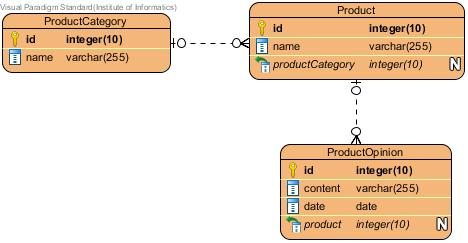
\includegraphics[width=0.6\textwidth]{erd}
\caption{\textit{ERD diagram of tested application model}}
\label{erd}
\end{figure}

\subsubsection{REST API} 
The tested application REST API provides the following resources:
\vspace{3mm}

\noindent\textbf{Find product category by ID} - returns product category with id defined by parameter \textit{id}.

  \begin{tabular}{ll}
  Method: & GET\\
  Path: & /find/\{id\}\\
  Parameters: & id (parameter type: path, data type: integer, required: yes)\\
  Response: & Product category in JSON format \\
  \end{tabular} \vspace{5mm}

\noindent\textbf{Add new product category} - creates new category with name defined by parameter \textit{categoryName}. For created category products with opinions are generated. Number of generated products and opinions is chosen randomly from range 1-4. 

  \begin{tabular}{ll}
  Method: & PUT \\
  Path: & /add/ \\
  Parameters: & categoryName (parameter type: request, data type: string, required: yes)\\
  Response: & Created product category in JSON format  \\
  \end{tabular} \vspace{5mm}

\noindent\textbf{Update product category} - updates category defined by parameter \textit{id} by name from parameter \textit{newName}. 

  \begin{tabular}{ll}
  Method: & POST \\
  Path: & /update/\{id\} \\
  Parameters: & id (parameter type: path, data type: integer, required: yes)\\
              & newName (parameter type: request, data type: string, required: yes)\\
  Response: & Updated product category in JSON format  \\
  \end{tabular} \vspace{5mm}

\noindent\textbf{Remove product category} - removes product category with related products and opinions for given \textit{id}.

  \begin{tabular}{ll}
  Method: & DELETE \\
  Path: & /remove/\{id\} \\
  Parameters: & id (parameter type: path, data type: integer, required: yes)\\
  Response: & No content  \\
  \end{tabular} \vspace{5mm}

\noindent\textbf{Get all product categories paged} - returns product categories with products and opinions for page defined by parameters \textit{page} and \textit{size}.

  \begin{tabular}{ll}
  Method: & GET \\
  Path: & /findPart/ \\
  Parameters: & page (parameter type: request, data type: integer, required: yes)\\
              & size (parameter type: request, data type: integer, required: yes)\\
  Response: & Product categories in JSON format  \\
  \end{tabular} \vspace{5mm}
  
\noindent\textbf{Get all product categories} - returns all product categories with products and opinions.

  \begin{tabular}{ll}
  Method: & GET \\
  Path: & /findAll/ \\
  Response: & Product categories in JSON format  \\
  \end{tabular} \vspace{5mm}
  
\noindent\textbf{Remove all product categories} - removes all product categories with related products and opinions.

  \begin{tabular}{ll}
  Method: & DELETE \\
  Path: & /removeAll/ \\
  Response: & No content  \\
  \end{tabular} \vspace{5mm}
  
\noindent\textbf{Create product categories} - generates number of product categories. The number is defined by \textit{size} parameter. For each category products with opinions are generated. Number of generated products and opinions is chosen randomly from range 1-4. 

  \begin{tabular}{ll}
  Method: & PUT \\
  Path: & /addCategories/ \\
  Parameters: & size (parameter type: request, data type: integer, required: yes)\\
  Response: & String message  \\
  \end{tabular} \vspace{5mm}

\noindent\textbf{Execute task} - starts task which will simulate high CPU usage. For that purpose generation of 40th number of Fibonacci sequence was chosen. 

  \begin{tabular}{ll}
  Method: & GET \\
  Path: & /task/ \\
  Response: & No content  \\
  \end{tabular} \vspace{2mm}
  
Services \textit{Find product category by ID}, \textit{Add new product category}, \textit{Update product category}, \textit{Remove product category} provides basic usage from client perspective. Remaining services was developed for testing purposes (performance tests for different configuration and redundant components from Chapter \ref{realization}).
  
\subsubsection{Implementation decisions} 
The application will be implemented in Java 1.8. Web based features will be implemented in Spring Framework 4.3.7 and Hibernate 5.0.12. The application server for the application will be Apache Tomcat 8.5.11 served by Spring Bootstrap 1.5.2. Data persistence will be realized with PostgreSQL 9.6 DBMS.  

Above tools are commonly used solutions in a web development. That fact makes implemented solution applicable and easily translated to other web applications based on similar technologies.  

\subsection{System Principles} \label{principles}
The key in every successful project is to define goals and needs at the beginning.
In case of this work it will be realized as system principles definition on the base of  performance problems from chapter \ref{PerformanceRelatedProblems}.

Downplaying of performance evaluation tests - decision of when, how often or even if perform performance evaluation tests lays in developers way of working. However, performance evaluation tests performed in easy way with minimal effort could encourage developer teams to perform it. 

Complexity of performance tuning - the system should know which set of configuration parameters values will be the best in given situation.  

Process of performance tuning is time consuming and manual - the system should know how to tune configuration to increase performance of application and do it automatically. 

Workload is various - the system should be able to monitor workload of application in form of incoming requests in order to switch application configuration which will be more suitable in given circumstances. 

On the base of above consideration following set of principles of the system can be formulated:

\begin{itemize}
\item The system should perform live monitoring of application
\item The system should be autonomous
\item The system should be able to perform configuration change during application runtime
\item The system should be able to work in production environment
\item The system should have minimal impact on production environment
\end{itemize}

On the base of above principles in the next chapter proposition of system realization will be introduced.  

\subsection{Performance Improvement Realization} \label{realization}

Before system architecture will be introduced a set of elements on which performance tuning will be performed must be introduced.  
Considering existing solutions presented in chapter \ref{ExistingSolutions} author of this work decided to perform performance tuning of the application on the base of two techniques: redundant components and application server configuration parameters. 

\subsubsection{Research Environment}

In order to make right choices about performance improvement realization a set of experiments must be performed. 
For that purpose 10000 product categories with related entities were generated. Each product category may have from 1 to 4 products. Each product may have from 1 to 4 opinions. Exact number of related entities was chosen randomly during generation. In summary number of created entities for experiments is as follows:
\begin{itemize}
\item Product category: 10000 entities
\item Product: 22269 entities
\item Product opinion: 49406 entities
\end{itemize}  

Execution time of methods was measured by aspect oriented class. The class wraps method by execution time measurement by calculation difference between two dates: start date (measured before method execution) and end date (measured after method execution). The execution time was logged and persisted in a time series database (InfluxDB) in order to enable further analysis. In order to make execution time more accurate each experiment was developed 10 times and final execution time was calculated as arithmetic mean of 10 values obtained in individual experiments. 

Required workload was simulated by tests scenarios generated in Gatling Load and Performance testing engine\cite{gatling}. Following test scenarios was developed:
\begin{itemize}
\item \textbf{Squeeze Application} - generates high CPU usage of the tested application by firing 100 parallel requests to CPU consuming resource - "Execute task". 
\item \textbf{Frequently Changing Model} - generates traffic with alternate firing  "Update product category" and "Find product category by ID" resources in 10 parallel requests.
\item \textbf{Immutable Model} - generates traffic based on "Find product category by ID" resource (without changes on data model) in 10 parallel requests.
\item \textbf{Insert} - generates 20 sequenced requests to "Add new product category" resource. 
\end{itemize}

Author of this work decided to took into consideration following candidates: paging, cache, batched inputs. The decision was based on facts that all of mentioned candidates are able to increase performance of the  tested application domain and it is possible to develop a switchable equivalent for given a candidate. 

In the first experiment different paging mechanism was analyzed. The execution time for each mechanism was measured by summing up execution time needed to retrieve all 10000 product categories from the tested application.   

In the second experiment cache influence on performance was analyzed. Methods "Update product category" and "Find product category by ID" where tested with and without cache enabled against scenarios: Frequently Changing Model and    Immutable Model. 

In the next experiment solution with batched inserts was tested. Batch with size equal to 10 entities was used. Total time of execution during scenario Insert was compared with solution without batch. 

The last experiment tested influence of number of threads used by application server. In order to simulate complex tasks execution by each thread Squeeze Application scenario was used against 2, 10, 25 and 100 threads. 

\subsubsection{Redundant Components}
Redundant components, by definition, provide the same services but with different implementation. From the performance perspective that idea can be used to implement component which will provide the same services with different performance characteristic. What is also important, usage of redundant components must be justified - there must exist circumstance where given redundant component will offer better performance than another redundant component. 

Paging is database query realization in which in a single select query only part (page) of records is returned instead of querying all records from database. Table \ref{pagingcomponents} shows comparison of two proposed redundant components: Paging and No Paging.  
\begin{table}[!htb]
\def\arraystretch{1.5}
\caption{\textit{Paging redundant components comparison}}\label{pagingcomponents}
\begin{tabularx}{\textwidth}{p{3cm}|X|X}
  \textbf{Category} &\textbf{Paging} & \textbf{No Paging} \\
\hline
Query all records & Multiple queries (slower) & One query (faster) \\
User satisfaction & High & Low\\
Top performance circumstances & When impossible to query all records by No Paging component & When possible to query all records at once\\
\end{tabularx}
\end{table}

\begin{figure}[!htb]
\centering
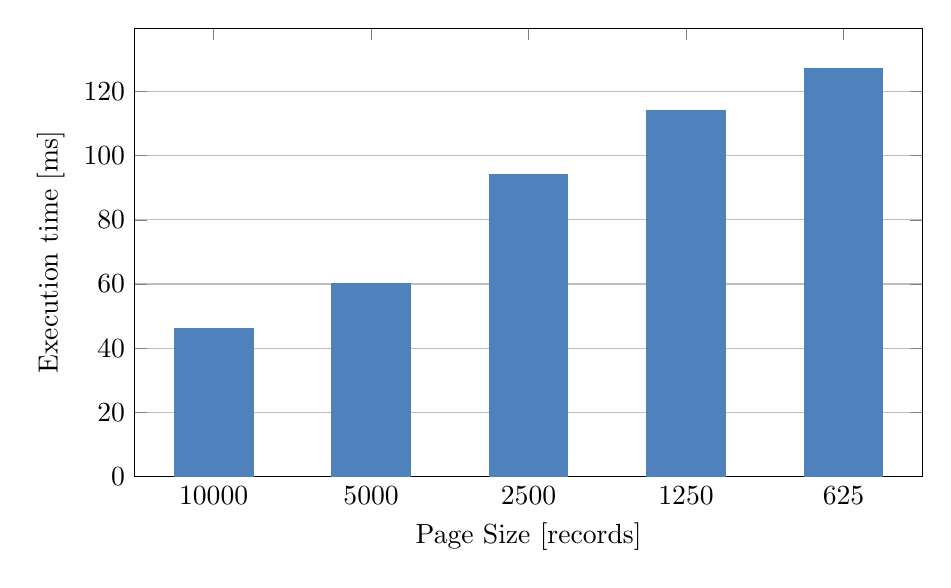
\begin{tikzpicture}
        \begin{axis}[
            symbolic x coords={{10000}, {5000}, {2500}, {1250}, {625}},
            xtick=data,
            bar width=1cm,
            x=2cm,
            ymin=0,
            enlarge x limits={abs=1cm},
            xlabel={Page Size [records]},
            ylabel={Execution time [ms]},
            ymajorgrids = true,
          ]
            \addplot[ybar,style={bblue,fill=bblue,mark=none}] coordinates {
                ({10000}, 46)
                ({5000},  60)
                ({2500},  94)
                ({1250},  114)
                ({625},   127)
            };
        \end{axis}
\end{tikzpicture}

\caption{\textit{Execution time comparison for different page sizes for 10000 product categories}} \label{fig:pagesizetime}

\end{figure}

As shown in Figure \ref{fig:pagesizetime} the bigger page size is, the smaller execution time is. It is related to fact that every query to a database generates additional overhead. 
In general the No Paging component is faster when it is possible to query all records at once. Possible to query means that query will not need more resources (memory, CPU) than is needed to be performed. 
The Paging component must perform multiple queries to a database in order to query all existing records. From the practical point of view in presentation layer only first page of records is needed when user entering a web page. Otherwise, long time of No Paging component execution will decrease user satisfaction level.  

The paging idea is more related to data presentation layer and user satisfaction. Moreover, when number of records in a database is possible to query at once No Paging component will be always faster to query all records. Because of that author of this work decided to reject paging as redundant component. 

Next redundant component candidate is cache. There exist many levels of abstraction on which cache can be applied to a web application - request level cache, method level cache, global data cache. For goals of this work method-level cache of service responsible for managing database operations was chosen - in general such operations are time consuming. The cache saves returned value from method and uses input parameters as cache key. Table \ref{cachecomponents} shows comparison of two proposed redundant components: Cache (methods are cached) and No Cache (cache is disabled).
\begin{table}[!htb]
\def\arraystretch{1.5}
\caption{\textit{Cache and No Cache redundant components comparison.}}\label{cachecomponents}
\begin{tabularx}{\textwidth}{p{6cm}|X|X}
  \textbf{Category} &\textbf{Cache} & \textbf{No Cache} \\
\hline
Preferable parameters characteristic & Repeatable & Varied \\
Preferable resources & Immutable & Mutable\\
Overhead & Yes & No\\
\end{tabularx}
\end{table}
 
Table \ref{cachecomponents} shows that Cache and No Cache redundant components have different characteristic. In workload in which requests are repeatable (given set of parameters is used more than once) and there are no frequent changes in state of requested resources (no updates and inserts into a database) preferred redundant component is Cache. When there is no repeatable requests and requested resources are frequently changed, usage of cache generates only additional overhead. In such cache No Cache component should be used. On the base of above considerations Cache/No Cache components could be considered as a proper redundant component from performance perspective and will be implemented in the system. 

Last redundant component taken into consideration are batched inserts. The idea is to gather objects which are to be inserted into a database and insert them in one query instead of few separate ones. This minimize query overhead. In case of this work inserts batch is realized in form of collection of the objects in which insert query is fired when collection is full.   
Table \ref{batchedcomponents} shows comparison of two proposed redundant components: Batched (records to insert are batched) and Direct (direct inserts into a database as separate queries).

\begin{table}[!htb]
\def\arraystretch{1.5}
\caption{\textit{Batched and Direct redundant components comparison.}}\label{batchedcomponents}
\begin{tabularx}{\textwidth}{p{4cm}|X|X}
  \textbf{Category} &\textbf{Batched} & \textbf{No Batched} \\
\hline
Query execution time & Faster & Slower \\
Query effects & Delayed & Instant\\
Efficiency & High & Low\\
\end{tabularx}
\end{table}

\begin{figure}[!htb]
\centering
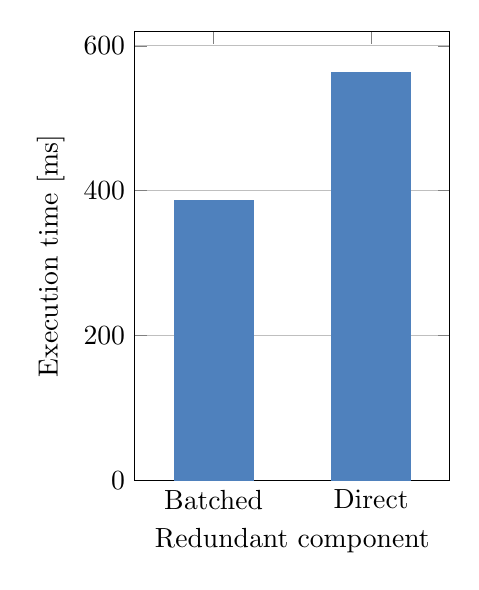
\begin{tikzpicture}
        \begin{axis}[
            symbolic x coords={Batched, Direct},
            xtick=data,
            bar width=1cm,
            x=2cm,
            ymin=0,
            enlarge x limits={abs=1cm},
            xlabel={Redundant component},
            ymajorgrids = true,
            ylabel={Execution time [ms]}
          ]
            \addplot[ybar,style={bblue,fill=bblue,mark=none}] coordinates {
                (Batched,  386)
                (Direct,   563)
            };
        \end{axis}
\end{tikzpicture}
\caption{\textit{Execution time comparison for Batched and Direct redundant components for batch with size = 10 and number of records = 20}} \label{fig:batchedtime}
\end{figure}

The components comparison in Table \ref{batchedcomponents} shows different characteristic of both redundant components. Batched one is in general more efficient and faster than No Batched. However, process of batching records introduces delays in real effect of batched statement (equal to time in which given records sf "frozen" in the batch). In proposed implementation batched statement will be fired when batch is full. Both facts lead to conclusion that Batched component should be used only in circumstances when such delay is acceptable by users or when number of inserts into a database is so high that efficiency improvement is needed. Another thing is the more frequent inserts into a database (faster filling up of batch) the smaller delay. Therefore Batched component should be used only in case when number of inserts into a database is very high. Otherwise Direct component should be used. Above considerations justify choice of Batched/Direct redundant components to be used in the system.   

\subsubsection{Application Server Configuration Parameters}

Configuration of application server is crucial for performance of application. Application servers provide wast number of parameters which can be configured. Such parameters may be slightly different depending from vendor but in most cases configuration provide possibility to adjust: thread number, JDBC connection pools, EJB pools, JVM configuration. 

Author of this work decided to take into consideration 2 possible configurations: EJB pool size and thread number of application server. Both configurations have direct influence on number of requests which are handled by application and should provide high performance improvements in the application domain. 

EJB pooling mechanism reduces time needed for creating new bean instances (beans are created on start up and kept in pool) and support parallel request handling. In case of this work tested application is developed in Spring framework with singleton scoped beans (there is one instance of bean for entire application) - therefore EJB pool configuration has no effect on application performance (singleton beans are not pooled). Influence of EJB pool size on performance of enterprise application was used up in other work \cite{autotuning} where authors already proved that tuning EJB pool size has positive influence on a JEE application performance. Taking into account this arguments EJB pool will be not implemented in the system. 

Number of threads has key meaning in handling incoming requests into an application server. When number of threads is less than a number of parallel incoming requests not handled part will be waiting in the queue until threads will be free again. Too large number of threads results in increased CPU usage and slower performance. This fact is documented in the Figure \ref{fig:threads}. For 100 incoming parallel requests three different configuration of thread number was tested: 1 thread, 10 threads, 100 threads. As one can see mean response time was high when too many parallel threads was executed or when number of threads was not sufficiently large to handle incoming requests.    

\pgfplotstableread[row sep=\\,col sep=&]{
    category           & t1    & t10    & t100  \\
    Min response time  & 1161.3  & 3549.8   & 33610.6 \\
    Max response time  & 85256 & 33587.1  & 37619.3 \\
    Mean response time & 43260.1 & 18705.5  & 36441.2 \\
    }\mydata
\begin{figure}[!htb]
\centering
\begin{tikzpicture}
    \begin{axis}[
            ybar,
            bar width=.6cm,
            width=\textwidth,
            height=.6\textwidth,
            legend style={at={(0.5,-0.15)},
                anchor=north,legend columns=-1},
            symbolic x coords={Min response time,Max response time,Mean response time},
            xtick=data,
            ymin=0,ymax=90000,
            ylabel={Execution time [ms]},
            enlarge x limits={abs=2cm},
            ymajorgrids = true,
        ]
        \addplot[style={bblue,fill=bblue,mark=none}] table[x=category,y=t1]{\mydata};
        \addplot[style={rred,fill=rred,mark=none}] table[x=category,y=t10]{\mydata};
        \addplot[style={ggreen,fill=ggreen,mark=none}] table[x=category,y=t100]{\mydata};
        \legend{1 thread, 10 threads, 100 threads}
    \end{axis}
\end{tikzpicture}
\caption{\textit{Mean response time from 100 incoming paraller requests}} \label{fig:threads}
\end{figure}


Number of threads has large impact on application performance and it configuration will be implemented in the system. 

\subsubsection{Performance Improvement Realization Summary}

Above considerations contain justification about accepted or declined candidates for performance tuning in the system. Finally, two redundant components (batched imports, cached methods) and one application server configuration parameter (threads number) was chosen.


\subsection{The System Architecture}

\subsubsection{Automated Performance Tuning System}

In order to enable performance tuning in the tested application on the base of solutions described in Chapter \ref{realization} the Automated Performance Tuning System (APTS) is introduced. The APTS is based on principles formulated in Chapter \ref{principles}. Main functionality of the system is to enable automated  performance tuning of the tested application in real time. 

\subsubsection{APTS Components}

As presented on Figure \ref{componentapts}, the system is composed of the following components: \textit{Workload Generator}, \textit{APTS Manager} which includes \textit{PET Cases} and \textit{Decision Module}, \textit{InfluxDB Service}, \textit{Configuration Service}, \textit{Resource Monitoring Service}, \textit{Aspect Oriented Application Monitoring} and \textit{Tested Application}.

\begin{figure}[!htb]
\centering
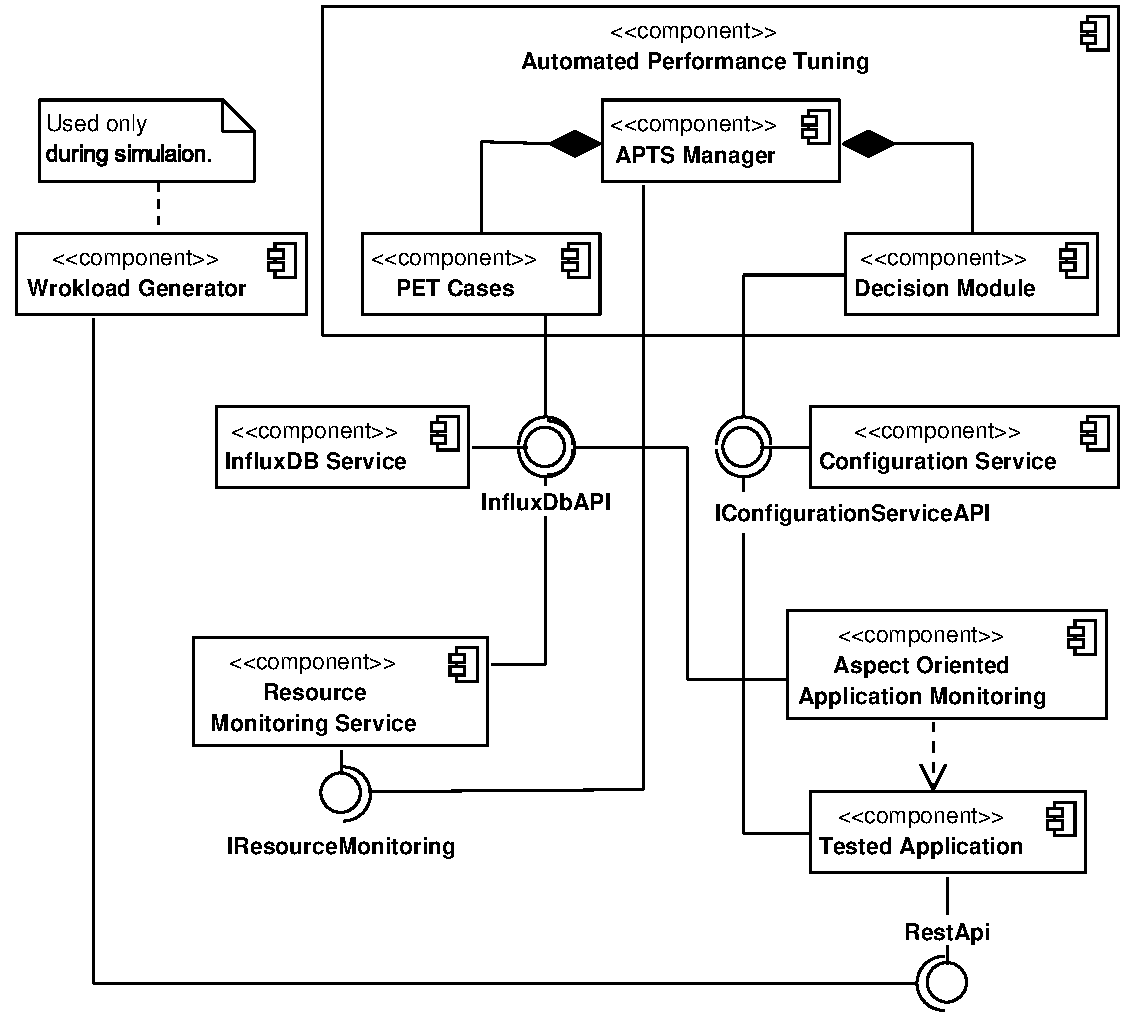
\includegraphics[width=1\textwidth]{APTSComponentDiagram}
\caption{\textit{Component diagram of the APTS}}
\label{componentapts}
\end{figure}

The goal of \textit{Workload Generator} is to provide simulation of network traffic to the tested application. Traffic simulation is realized as HTTP requests generation based on Gatling library \cite{gatling}. The \textit{Workload Generator} is independent from the APTS and it communicates directly to the tested application. Thank to that features the module can be easily disabled in production environment where real traffic is analyzed.  

The \textit{APTS Manager} is the main part of the system. It is responsible for enabling performance tuning by performing performance evaluation tests and reporting performance issues raised by tests to \textit{Decision Module}. 

The \textit{PET Cases} component contains performance evaluation scenarios written with help of PET Framework (see Chapter \ref{framework}). The tests monitor the tested application in specified schedule, gather monitored KPIs from \textit{InfluxDB Service} and asserts KPIs values. In case of failed assertion performance issue is raised.

The \textit{Decision Module} is responsible for performance issue analysis and performance tuning. This feature is realized in the form of rule based system in which performance issues are conditions and performance tuning decisions are actions.   

The \textit{InfluxDB Service} hosts InfluxDB \cite{influxdb} time series database which provides HTTP API for querying and writing data. The database stores performance measurements which are generated by the tested applications and required by the performance evaluation tests. In order to visualize data stored in the database in the form of readable graphs the Grafana \cite{grafana} platform was integrated with the InfluxDB. 

The \textit{Configuration Service} is an external service where performance tuning configuration is stored (active redundant component and current application server thread number). The \textit{Configuration Service} provides REST API which enables different parts of the system to check and change current configuration of the tested application.

The \textit{Resource Monitoring Service} is responsible for providing information about current resource consumption of the machine on which the \textit{Tested Application} is stored. The component is managed by the \textit{APTS Manager} which starts monitoring by sending HTTP request when performance evaluation tests are started. When the tests are finished monitoring is stopped by the manager by sending HTTP request. Data about resources consumption are written into the \textit{InfluxDB Service} in real time. 

The \textit{Aspect Oriented Application Monitoring} provides information about execution time of methods provided by the \textit{Tested Application} REST API. Since the monitoring is implemented in Spring Aspect Oriented Programming \cite{springaop} it is transparent for the \textit{Tested Application} - in other words - the \textit{Tested Application} does not know about the monitoring component. Informations about execution time are stored in the \textit{InfluxDB Service}.

The \textit{Tested Application} component represents the tested application described      wider in Chapter \ref{testedApplicaiotn}.


\subsubsection{APTS Deployment}

The system, as presented on Figure \ref{deploymentapts}, is deployed on \textit{Client Workstation}, \textit{Application Server} and \textit{Service Server}.

\begin{figure}[!htb]
\centering
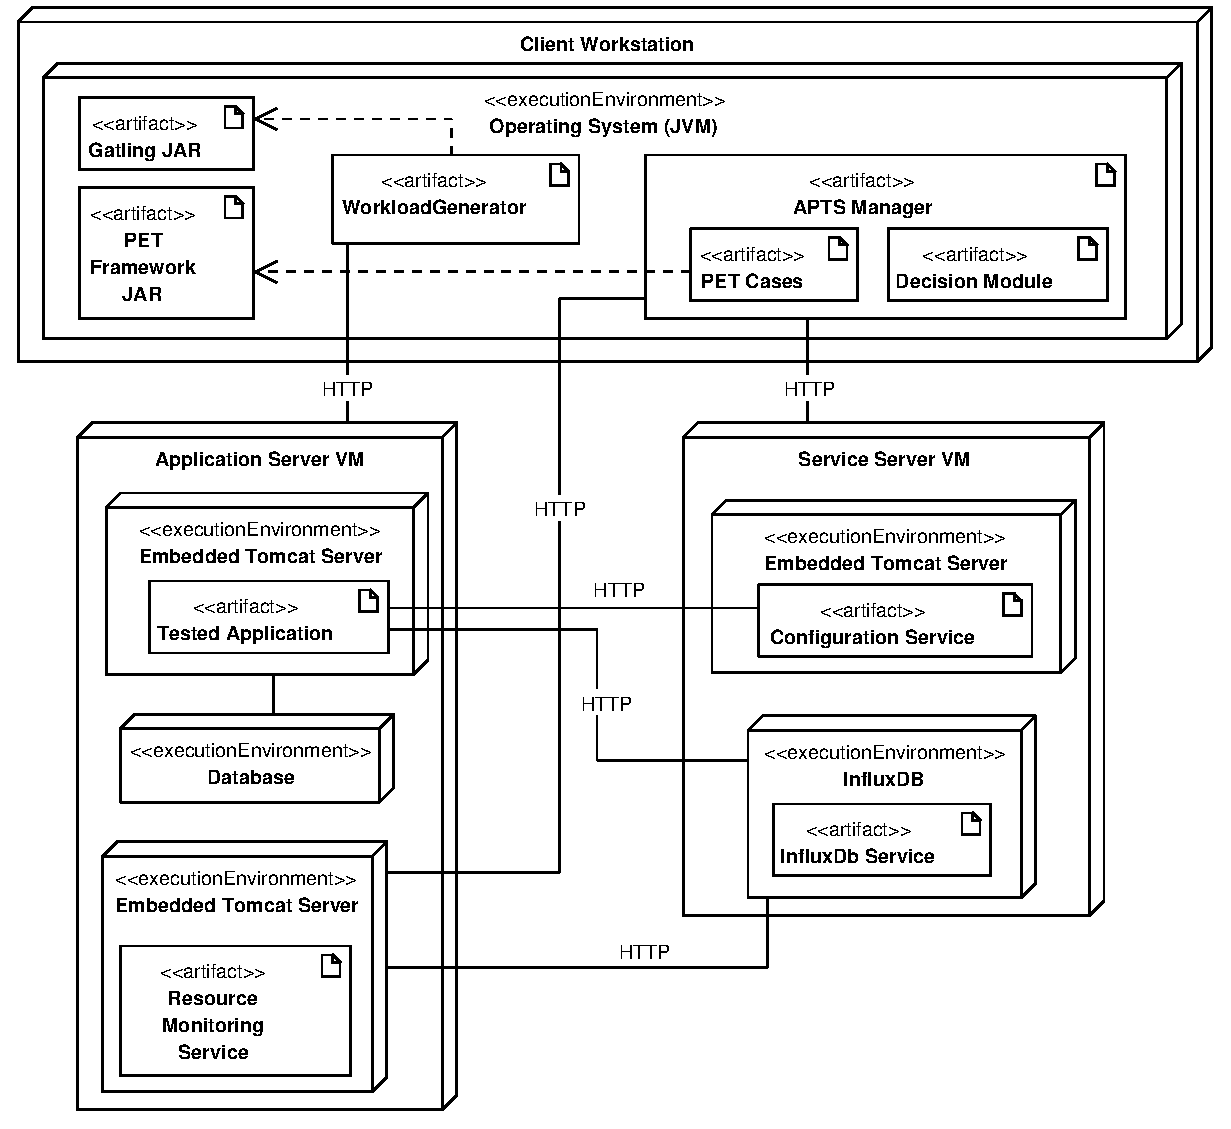
\includegraphics[width=1\textwidth]{APTSDeploymentDiagram}
\caption{\textit{Deployment diagram of the APTS}}
\label{deploymentapts}
\end{figure}



The \textit{Application Server} node is designated to host tested application and is independent from the rest of the system - in case of \textit{Configuration Server} unavailability predefined default configuration is used. When \textit{InfluxDB} is offline no performance measurements are stored. In order to provide information about current resource consumption on the node the \textit{Resource Monitoring} service is also deployed on the node. 

The \textit{Service Server} node holds additional services used by the APTS. This node was separated from the \textit{Application Server} node in order to minimize overhead of the APTS on the tested application.

The node called \textit{Client Workstation} is any node (with JRE installed) which holds the \textit{APTS Manager}. 


\subsubsection{PET Framework} \label{framework}
 
In order to implement performance evaluation tests cases in readable, consistent and easy way the PET Framework was implemented. The framework is independent from the APTS what means that JAR with the framework can be used in any other project. 

The framework main features are:
\begin{itemize}
\item POJO based
\item PET cases configured by annotation
\item PET cases schedule
\item Performance issues reporting at runtime 
\item Test cases written in JUnit \cite{junit} style
\end{itemize}

Work with the framework is based on POJOs which provides lightness (no additional third party software or middleware is required) and flexibility (any Java code can be used during work with the framework) of the solution. PET cases are  configured using Java annotations what makes configuration readable and convenient. Each PET case is run in configured schedule what enables continuous monitoring of a tested software. Thanks to asynchronous implementation any issues which are reported during tests can be obtained immediately when appear. PET cases convention was inspired on popular and successful JUnit Framework - each person familiar with JUnit should easily understand conventions of PET Framework.       

Main elements on which PET Framework is based are annotations, assertions and performance issues. 

Annotations are used to mark POJOs to be interpreted as PET cases and to configure test case. In the PET Framework two annotations are available:

\begin{table}[!htb]
\def\arraystretch{1.5}
\begin{tabularx}{\textwidth}{p{1.4cm}X}
\textbf{@Pet} 	  & Annotation used to mark class to be interpreted as PET case container. \\ 
\textbf{@PetCase} & Annotation used to mark method to be interpreted as PET case. Available parameters are presented in the Table \ref{petcase}. To explain parameters more deeply lets consider example in which parameters are configured as follows: \textit{monitorIntervalInSec} = 30, \textit{durationInSec} = 120. This values means that test case will be executed in every 30 seconds in period of time equal to 120 seconds (2 minutes) i.e., a test case will be executed 4 times and after 2 minutes execution will terminate. Assuming that a test case will be started at 12:00:00 hour, executions will be started at 12:00:00, 12:00:30, 12:01:00 and 12:01:30. 
\end{tabularx}
\end{table}

\begin{table}[!htb]
\def\arraystretch{1.5}
\caption{\textit{Available parameters of @PetCase annotation}}\label{petcase}
\begin{tabularx}{\textwidth}{p{3.1cm}|p{1.3cm}|p{1.1cm}|X}
  \textbf{Parameter name} &\textbf{Type} & \textbf{Default value} & \textbf{Description} \\
\hline
			\textit{enabled} & boolean & true & Indicates if PET case should be run.\\
			\textit{monitorIntervalInSec} & integer & 30 & Interval between test case executions in seconds.\\
			\textit{durationInSec} & integer & 3600 & Maximum duration of the test case in seconds.\\
			\textit{delayInSec} & integer & 0 & Delay after which the tests case will start in seconds.\\
\end{tabularx}
\end{table}			

In order to evaluate current KPIs against specified values a set of assertion was introduced. In case of assertion failure PET Framework convert exception to the performance issue. Signatures of assertions are presented on Listing  \ref{assertions}. As presented, for the performance evaluation tests three assertions where implemented (to ensure that KPI is less, greater of equal to specified value).  Parameters used in assertions are: 
\begin{itemize} 
\item \textit{metric} - identifier of KPI used in performance issue.
\item \textit{currentValue} - current value of KPI measured on an tested application
\item \textit{limit}/\textit{expectedValue} - value to which currentValue is compared to. In case when limit is exceeded or value is different than expected assertion error is thrown.
\end{itemize}

\begin{listing}[ht]\begin{minted}[fontsize=\footnotesize]{java}

void assertKpiLessThan(String metric, Double currentValue, Double limit);

void assertKpiGreaterThan(String metric, Double currentValue, Double limit);

void assertKpiEqual(String metric, Double currentValue, Double expectedValue);
\end{minted}
\caption{PET assertions signatures} \label{assertions}
\end{listing}

Important part of the PET Framework is the Performance Issue entity. When PET assertion fails or monitoring state need to be announced the entity Performance Issue containing all necessary information about failure is used. Informations contained in Performance Issue entity are later analyzed by the Decision Module. Class diagram of the Performance Issue is presented on the Figure \ref{issue}.

\begin{figure}[!htb]
\centering
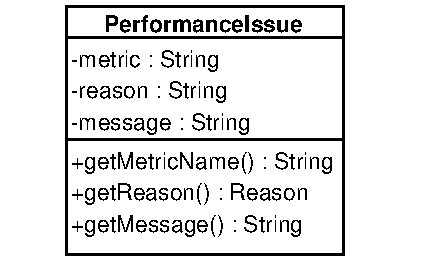
\includegraphics[width=0.45\textwidth]{PerformanceIssueClassDiagram}
\caption{\textit{PerformanceIssue class diagram}} \label{issue}
\end{figure}
 
Attributes of the class are: 
\begin{itemize}
\item \textit{metric} - identified of monitored KPI.
\item \textit{reason} - information about reason why issue is reported or current state of monitored KPI.
\item \textit{message} - human readable message with explanation about issue.
\end{itemize}

Sample PET case written with usage of the PET Framework is presented on the Listing \ref{case}. Annotations \textit{@Pet} and \textit{@PetCase} are used to inform framework that this class is implementation of PET case. Method  \textit{meanExecutionTimeShouldBeOnAcceptableLevel} is interpreted as PET case implementation and is configured by annotation \textit{@PetCase} with definied two attributes - \textit{monitorIntervalInSec} with assigned value 60 and \textit{durationInSec} with assigned value 3600. This configuration means that PET case will be executed in every minute by the period of 1 hour. In the body of the method assertion \textit{assertKpiIsLessThan} is defined which simply checks if mean execution time was on acceptable level - below 1.2 second. For simplicity process of retrieving execution time measurement was represented as method  \textit{getExecutionTimeFromLastMinute()}.  


\begin{listing}[ht]\begin{minted}[fontsize=\footnotesize]{java}
/*
 * imports
 */
@Pet
public class SamplePETCase {

    @PetCase(monitorIntervalInSec = 60, durationInSec = 3600)
    public void meanExecutionTime_shouldBeOnAcceptableLevel() throws Exception {
        
        double acceptableExecutionTime = 1200.;
        
        double meanExecutionTime = getExecutionTimeFromLastMinute();
        
        assertKpiLessThan(
            "executionTime", meanExecutionTime, acceptableExecutionTime
        );
    }
}
\end{minted}
\caption{Sample PET case written in the PET Framework} \label{case}
\end{listing}

In order to run tests cases the PET Framework provides runner (PetCaseRunner) which will run all tests cases marked with proper annotations from the give package. Because of the need of continuous monitoring of the reported performance issues, the runner is implemented as a thread and provides asynchronous API to retrieve new reported issues. The Listing \ref{petrunner} presents sample usage of the PetCaseRunner. 

\begin{listing}[ht]\begin{minted}[fontsize=\footnotesize]{java}
PetCaseRunner runner = new PetCaseRunner("com.zalas.masterthesis.apts.pet.cases");
runner.start();

while(runner.isAlive()) {
    Thread.sleep(1000);
    System.out.println(runner.getNewIssues());
}
\end{minted}
\caption{Sample usage of the PetCaseRunner} \label{petrunner}
\end{listing}

As presented on the Listing \ref{petrunner}, new instance of PetCaseRunner class is created. The package name where tests cases are located is given as a parameter to the constructor. Next, the instance of the runner is started - new thread is started. All PET cases are run on the defined schedule within this thread. In order to retrieve information about performance issues reported by test cases which are run by runner thread method \textit{getNewIssues()} is called within while loop in 1 second interval. In this sample usage retrieved issues are printed out to standard output. In case of APTS performance issues are delegated to the Decision Module where are analyzed. When all test cases are finished the runner thread is terminated.    

\subsubsection{Implemented PET Cases} \label{dm}

 The performance evaluation tests cases in the APTS are responsible for monitoring current state (execution time, resource consumption) of the tested application and reporting performance issues which are analyzed by the \textit{Decision Module}. The monitoring is realized on the base of data gathered in the \textit{InfluxDB Service}.  Tuning of the tested application is realized using elements chosen in the Chapter \ref{realization}. In order to enable tuning of the considered elements from the Chapter \ref{realization} following PET cases was implemented: \textit{MeanExecutionTimePET}, \textit{MonitorInsertsLevelPET},  \textit{MonitorTrafficProfilePET}.
 
 The \textit{MeanExecutionTimePET} test case monitors mean execution time from given interval of the methods provided by the tested application REST API. If mean execution time is greater than specified value the performance issue is reported. 

The \textit{MonitorInsertsLevelPET} test case monitors how many database inserts are performed on the tested application. If number of inserts per seconds is greater the a given threshold the reported performance issue contains information about high level of inserts. Otherwise, the performance issue contains information about low level of inserts. The performance issue with above information is reported after every execution of test case. 

The \textit{MonitorTrafficProfilePET} test case monitors traffic profile which comes to the tested application. There are two possible values of traffic profile - mutable and immutable. A mutable traffic profile means that state of the tested application is changed (by inserts or updates operations). An immutable traffic profile means that requests to the application do not change state of the tested application (read requests). The traffic profile is considered as immutable when number of immutable requests is greater than mutable requests. The performance issue with information about traffic profile is reported after every execution of test case.

\begin{table}[!htb]
\def\arraystretch{1.5}
\caption{\textit{Possible values of the Performance Issue reported by the specific test case.}}\label{testcasescomp}
\begin{tabularx}{\textwidth}{X|X|p{3.8cm}}
\textbf{Test Case} & \textbf{Metric Name of Performance Issue} & \textbf{Possible Reasons of Performance Issue} \\ \hline
MeanExecutionTimePET & executionTime & EXCEEDED \\\hline
MonitorInsertsLevelPET & insertsLevel &LOW, HIGH \\\hline
MonitorTrafficProfilePET & trafficProfile & MUTABLE, IMMUTABLE \\
\end{tabularx}
\end{table}

\subsubsection{Decision Module} \label{dm}

The role of the \textit{Decision Module} is to perform performance tuning actions on the base of reported performance issues, current configuration of the tested application and current resource consumption on the node where the tested application is deployed (see the Figure \ref{decisionmodule}). 

\begin{figure}[!htb]
\centering
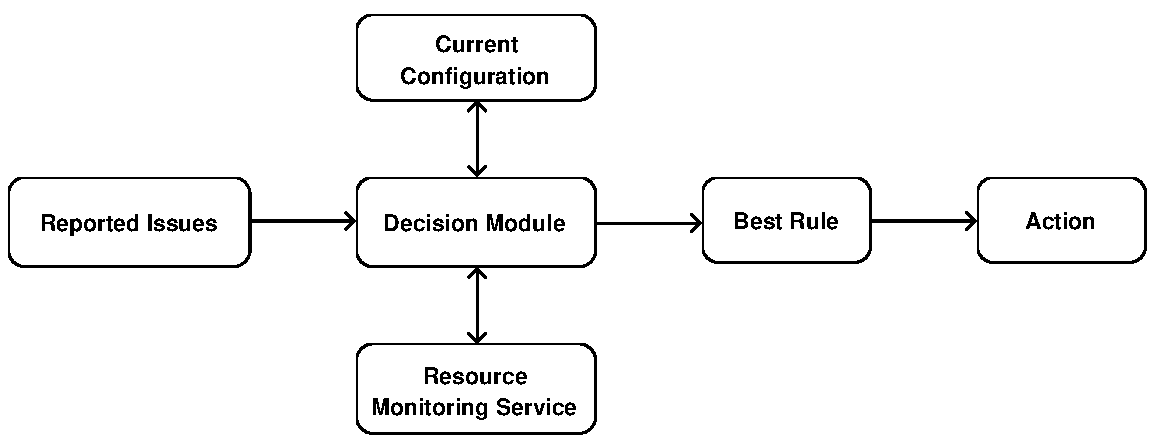
\includegraphics[width=0.9\textwidth]{DecisionModuleDiagram}
\caption{\textit{Performing Tuning Action by Decision Module}} \label{decisionmodule}
\end{figure}

Decision module is triggered by a reported performance issues in order to analyze above factors and perform action. Then, the \textit{Decision Module} retrieves information about current configuration of the tested application and resource consumption on the tested application node from \textit{Configuration Service} and \textit{Resource Monitoring Service}. Next, a decision about the best rule is preformed and action related to the best rule is executed (see the Figure \ref{dmsequence}). 

\begin{figure}[!htb]
\centering
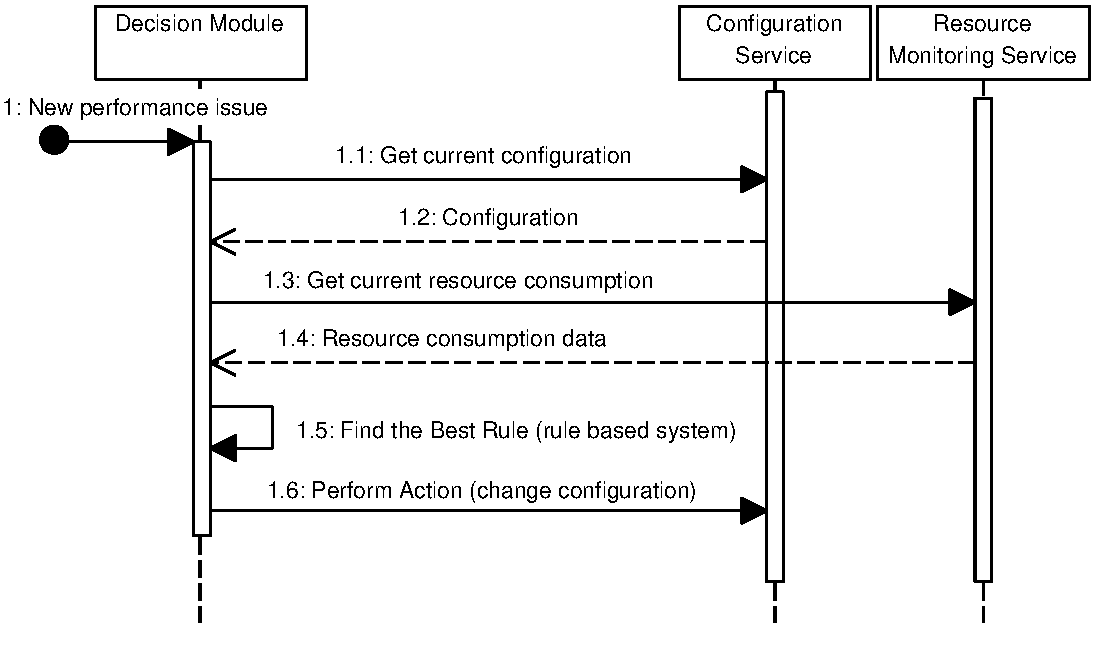
\includegraphics[width=1\textwidth]{DecisionModuleSequenceDiagram}
\caption{\textit{Sequence diagram presenting the Decision Module workflow}} \label{dmsequence}
\end{figure}

Decision about which action will be performed is made using a rule based system. Implemented rule based system is consist of two parts: set of the rules and inference engine. The set of rules is created with the aim of performance tuning of the tested application. Each rule fulfill contract defined in the form of the \textit{Rule} interface presented on the Listing \ref{irule}.

\begin{listing}[ht]\begin{minted}[fontsize=\footnotesize]{java}
public interface Rule {
    boolean isRuleApplicable(
    	IssueToHandle issueToHandle, 
    	ApplicationConfiguration currentConfiguration
    );
    void executeAction();
    int getPriority();
}
\end{minted}
\caption{Rule interface} \label{irule}
\end{listing}

The interface enforce on rules to define the following methods: 
\begin{itemize}
\item isApplicable - method evaluates boolean condition in order to decide if current rule is applicable for the reported performance issue.   
\item executeAction - action to perform when given rule is typed by the system as the best rule.   
\item getPriority - method returns priority of a given rule - the higher number - the higher priority.  
\end{itemize}

In order to perform automated tuning of the tested application based on elements defined in the Chapter \ref{realization} the following rules are implemented: \textit{Enable Batch Rule}, \textit{Disable Batch Rule}, \textit{Enable Cache Rule}, \textit{Disable Cache Rule}, \textit{Switch To 20 Threads Rule}, \textit{Switch To 50 Threads Rule}, \textit{Switch To 80 Threads Rule}. Below, all implemented rules are presented in details.  

\vspace{5mm}

%-------------ENABLE BATCH RULE START-----------------
\noindent\textbf{Enable Batch Rule} \\
The rule enables batching mechanism provided by the Batched redundant component in the tested application when the number of  inserts performed by the tested application is classified by the MonitorIsertsLevelPET test case as "high". Enabling batch mechanism should decrease total time of insert requests. Details of the rule are presented in the Table \ref{ruleenablebatch}.

\begin{table}[!htb]
\def\arraystretch{1.5}
\caption{\textit{Details of the Enable Batch Rule}} \label{ruleenablebatch}
\begin{tabularx}{\textwidth}{p{2.1cm}|X}

\textbf{Applicability Condition:} & \textbf{isIssueRelatedInsertsLevel} \textit{AND} \newline
\textbf{isInsertsLevelHigh} \textit{AND} \newline
\textbf{isBatchDisabled} \\ \hline

\textbf{Subconditions Definition:} & \textbf{isIssueRelatedInsertsLevel} -  Reported performance issue metric is equal to "InsertsLevel"  \\
& \textbf{isInsertsLevelHigh} - Reported performance issue status is equal to "High" \\
& \textbf{isBatchDisabled} - Current application configuration parameter "BATCH" is equal to "DIRECT" \\ \hline

\textbf{Action:} & Change the configuration of parameter "BATCH" to value "BATCHED" \\ \hline
\textbf{Priority:} & 1\\
\end{tabularx}
\end{table}

%-------------ENABLE BATCH RULE END-----------------
\vspace{5mm}
%-------------DISABLE BATCH RULE START-----------------
\noindent\textbf{Disable Batch Rule} \\
The rule disables batching mechanism provided by Batched redundant component. Instead, the Direct redundant component is used.  The rule is applicable when the number of inserts performed by the tested application is classified by the MonitorIsertsLevelPET test case as "low". Disabling batch mechanism should reduce delay introduced by the batch mechanism and provide instant insert into the database. Details of the rule are presented in the Table \ref{ruledisablebatch}.

\begin{table}[!htb]
\def\arraystretch{1.5}
\caption{\textit{Details of the Disable Batch Rule}} \label{ruledisablebatch}
\begin{tabularx}{\textwidth}{p{2.1cm}|X}

\textbf{Applicability Condition:} & \textbf{issueRelatedToInsertsLevel} \textit{AND} \newline
\textbf{isInsertsLevelLow} \textit{AND} \newline
\textbf{isBatchEnabled} \\ \hline

\textbf{Subconditions Definition:} & \textbf{issueRelatedToInsertsLevel} -  Reported performance issue metric equals to "InsertsLevel"  \\
& \textbf{trafficProfileIsLow} - Reported performance issue status is equal to "Low" \\
& \textbf{batchAlreadyEnabled} - Current application configuration parameter "BATCH" is equal to "BATCHED" \\ \hline

\textbf{Action:} & Change the configuration of parameter "BATCH" to value "DIRECT"\\ \hline
\textbf{Priority:} & 1\\
\end{tabularx}
\end{table}
%-------------DISABLE BATCH RULE END-----------------
\vspace{5mm}
%-------------ENABLE CACHE RULE START-----------------
\noindent\textbf{Enable Cache Rule} \\
The rule enables cache mechanism provided by the Cache redundant component in the tested application when traffic profile incoming to the tested application is classified by the MonitorTrafficProfilePET test case as "immutable". Enabling cache mechanism should decrease time of requests execution. Details of the rule are presented in the Table \ref{ruleenablecache}.

\begin{table}[!htb]
\def\arraystretch{1.5}
\caption{\textit{Details of the Enable Chache Rule}} \label{ruleenablecache}
\begin{tabularx}{\textwidth}{p{2.1cm}|X}

\textbf{Applicability Condition:} & \textbf{isIssueRelatedTrafficProfile} \textit{AND} \newline
\textbf{isTrafficImmutable} \textit{AND} \newline
\textbf{isCacheDisabled} \\ \hline

\textbf{Subconditions Definition:} & \textbf{isIssueRelatedTrafficProfile} -  Reported performance issue metric is equal to "TrafficProfile"  \\
& \textbf{isTrafficImmutable} - Reported performance issue status is equal to "Immutable" \\
& \textbf{isCacheDisabled} - Current application configuration parameter "CACHE" is equal to "NO\_CACHE" \\ \hline

\textbf{Action:} & Change the configuration of parameter "CACHE" to value "CACHED" \\ \hline
\textbf{Priority:} & 1\\
\end{tabularx}
\end{table}
%-------------ENABLE CACHE RULE END-----------------
\vspace{5mm}
%-------------DISABLE CACHE RULE START-----------------
\noindent\textbf{Disable Cache Rule} \\
The rule disables cache mechanism provided by the Cache redundant component. Instead the  No Cache redundant component is used. The rule is applicable when traffic profile incoming to the tested application is classified by the MonitorTrafficProfilePET test case as "mutable". Disabling cache mechanism should eliminate overhead related to the cache mechanism which in mutable environment is needless. Details of the rule are presented in the Table \ref{ruledisablecache}.

\begin{table}[!htb]
\def\arraystretch{1.5}
\caption{\textit{Details of the Disable Cache Rule}} \label{ruledisablecache}
\begin{tabularx}{\textwidth}{p{2.1cm}|X}

\textbf{Applicability Condition:} & \textbf{isIssueRelatedTrafficProfile} \textit{AND} \newline
\textbf{isTrafficMutable} \textit{AND} \newline
\textbf{isCacheEnabled} \\ \hline

\textbf{Subconditions Definition:} & \textbf{isIssueRelatedTrafficProfile} -  Reported performance issue metric is equal to "TrafficProfile"  \\
& \textbf{isTrafficMutable} - Reported performance issue status is equal to "Mutable" \\
& \textbf{isCacheEnabled} - Current application configuration parameter "CACHE" is equal to CACHED" \\ \hline

\textbf{Action:} & Change the configuration of parameter "CACHE" to value "NO\_CACHE" \\ \hline
\textbf{Priority:} & 1\\
\end{tabularx}
\end{table}
%-------------DISABLE CACHE RULE END-----------------
\vspace{5mm}
%-------------SWITCH TO 20 THREADS RULE START-----------------
\noindent\textbf{Switch to 20 Threads Rule} \\
The rule represents the lowest possible threads number available in the APTS implementation. The rule switches configuration responsible for the number of threads used by application server on which the tested application is deployed to 20 threads. The rule is applicable when mean execution time defined in MeanExecutionTimePET test case is exceeded and CPU usage on the application node is high.  Switching to low threads number should help reduce CPU usage and hence reduce total execution time of the requests. Details of the rule are presented in the Table \ref{rules20}.

\begin{table}[!htb]
\def\arraystretch{1.5}
\caption{\textit{Details of the Switch to 20 Threads Rule}} \label{rules20}
\begin{tabularx}{\textwidth}{p{2.1cm}|X}

\textbf{Applicability Condition:} & \textbf{isExecutionTimeExceeded} \textit{AND} \newline
\textbf{isThreadsNumberDifferent} \textit{AND} \newline
\textbf{cpuUsageIsHigh} \\ \hline

\textbf{Subconditions Definition:} & \textbf{isExecutionTimeExceeded} -  Reported performance issue metric is equal to "ExecutionTime"  \\
& \textbf{isThreadsNumberDifferent} -  Current application configuration parameter "THREADS" is not equal to "T20" \\
& \textbf{cpuUsageIsHigh} - Current CPU usage on the application node is greater than 80\% \\ \hline

\textbf{Action:} & Change the configuration of parameter "THREADS" to value "T20" \\ \hline
\textbf{Priority:} & 1\\
\end{tabularx}
\end{table}
%-------------SWITCH TO 20 THREADS END-----------------
\vspace{5mm}
%-------------SWITCH TO 50 THREADS RULE START-----------------
\noindent\textbf{Switch to 50 Threads Rule} \\
The rule represents the middle possible value of threads number available in the APTS implementation. The rule switches configuration responsible for the number of threads used by application server on which the tested application is deployed to 50 threads. Conditions of applicability of rule are as following: mean execution time defined in MeanExecutionTimePET test case is exceeded and CPU usage is high or low for respectively low or high threads number. Switching to the higher threads number should help reduce execution time of requests which are waiting in the queue to be handled by the application. Switching to the lower threads number should help reduce CPU usage and hence reduce total execution time of the requests. In order to perform threads number switching by one level the rule has set higher priority in comparison to other threads related rules (in example: when current thread number is 20, and rules "Switch to 50 Threads Rule" and "Switch to 80 Threads Rule" are evaluated as applicable - rule "Switch to 50 Threads Rule" will be choose because of the higher priority). Details of the rule are presented in the Table \ref{rules50}.

\begin{table}[!htb]
\def\arraystretch{1.5}
\caption{\textit{Details of the Switch to 80 Threads Rule}} \label{rules50}
\begin{tabularx}{\textwidth}{p{2.1cm}|X}

\textbf{Applicability Condition:} & \textbf{isExecutionTimeExceeded} \textit{AND} \newline
(\textbf{isThreadNumber20} \textit{AND} \textbf{cpuUsageIsLow}) \textit{OR} \newline
(\textbf{isThreadNumber80} \textit{AND} \textbf{cpuUsageIsHigh}) \\ \hline

\textbf{Subconditions Definition:} & \textbf{isExecutionTimeExceeded} -  Reported performance issue metric is equal to "ExecutionTime"  \\
& \textbf{isThreadNumber20} -  Current application configuration parameter "THREADS" is equal to "T20" \\
& \textbf{isThreadNumber80} -  Current application configuration parameter "THREADS" is equal to "T80" \\
& \textbf{cpuUsageIsLow} - Current CPU usage on the application node is not greater than 80\% \\ \hline
& \textbf{cpuUsageIsHigh} - Current CPU usage on the application node is greater than 80\% \\ \hline

\textbf{Action:} & Change the configuration of parameter "THREADS" to value "T50" \\ \hline
\textbf{Priority:} & 2\\
\end{tabularx}
\end{table}
%-------------SWITCH TO 50 THREADS END-----------------

\vspace{5mm}
%-------------SWITCH TO 80 THREADS RULE START-----------------
\noindent\textbf{Switch to 80 Threads Rule} \\
The rule represents the highest possible threads number available in the APTS implementation. The rule switches configuration responsible for the number of threads used by application server on which the tested application is deployed to 80 threads. The rule is applicable when mean execution time defined in MeanExecutionTimePET test case is exceeded and CPU usage on the application node is low. Switching to high threads number should help reduce execution time of requests which are waiting in the queue to be handled by the application. Details of the rule are presented in the Table \ref{rules80}.

\begin{table}[!htb]
\def\arraystretch{1.5}
\caption{\textit{Details of the Switch to 80 Threads Rule}} \label{rules80}
\begin{tabularx}{\textwidth}{p{2.1cm}|X}

\textbf{Applicability Condition:} & \textbf{isExecutionTimeExceeded} \textit{AND} \newline
\textbf{isThreadsNumberDifferent} \textit{AND} \newline
\textbf{cpuUsageIsLow} \\ \hline

\textbf{Subconditions Definition:} & \textbf{isExecutionTimeExceeded} -  Reported performance issue metric is equal to "ExecutionTime"  \\
& \textbf{isThreadsNumberDifferent} -  Current application configuration parameter "THREADS" is not equal to "T80" \\
& \textbf{cpuUsageIsLow} - Current CPU usage on the application node is not greater than 80\% \\ \hline

\textbf{Action:} & Change the configuration of parameter "THREADS" to value "T80" \\ \hline
\textbf{Priority:} & 1\\
\end{tabularx}
\end{table}
%-------------SWITCH TO 80 THREADS END-----------------

\vspace{10mm}
%-------------DO NOTHING RULE START-----------------
\noindent\textbf{Do Nothing Rule} \\
The rule is returned by the implemented rule based system when there is no applicable rules for the current system state.  The rule is created as consequence of the Null Object Pattern \cite{nop} usage in the implementation of the system and is not stored in the set of available rules of the rule based system. Execution of the rule does not change anything - implementation of the method \textit{executeAction()} is empty. Details of the rule are presented in the Table \ref{ruledonothing}.

\begin{table}[!htb]
\def\arraystretch{1.5}
\caption{\textit{Details of the Do Nothing Rule}} \label{ruledonothing}
\begin{tabularx}{\textwidth}{p{2.1cm}|X}

\textbf{Applicability Condition:} & N/A \\ \hline

\textbf{Action:} & N/A \\ \hline
\textbf{Priority:} & 0\\
\end{tabularx}
\end{table}
%-------------DO NOTHING THREADS END-----------------

\pagebreak


Second part of the implemented rule based system is inference engine. The role of the engine is to choose the best rule from the set of provided rules and perform action related to chosen rule. In order to achieve this the algorithm presented in the Figure \ref{dmalgorithm} is used. 

\begin{figure}[!htb]
\centering
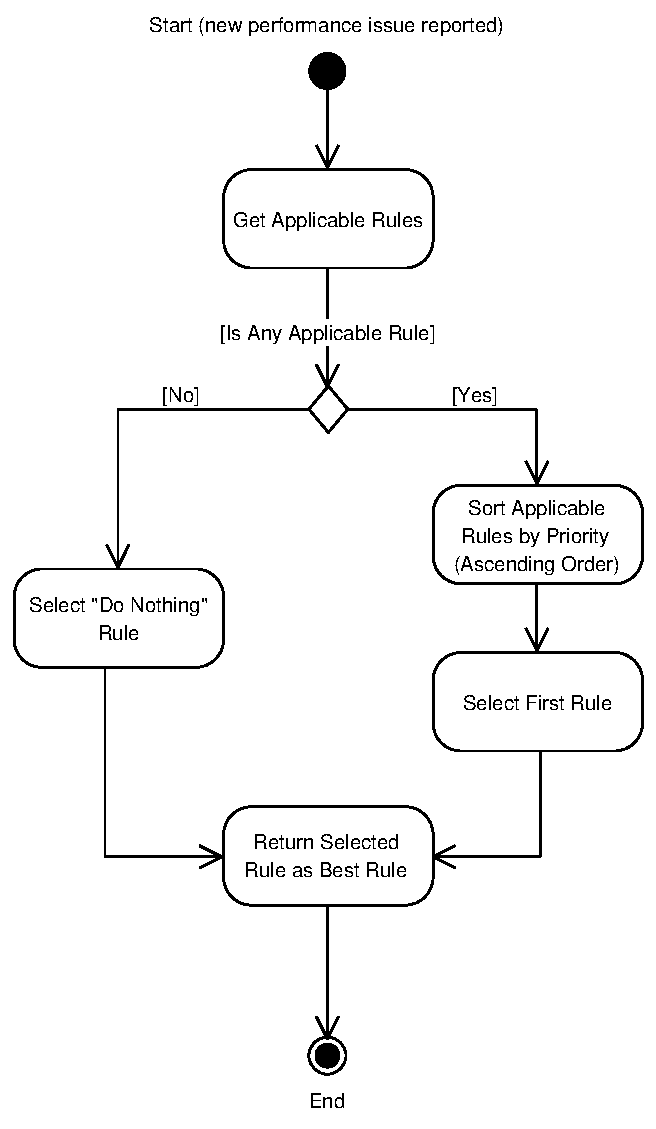
\includegraphics[width=0.55\textwidth]{DecisionModuleActivityDiagram}
\caption{\textit{The algorithm of selecting best rule by implemented rule based system}} \label{dmalgorithm}
\end{figure}

First step of the algorithm is to choose only applicable rules from the set of rules. In case when there are applicable rules - rule with the highest priority is chosen as best rule. If there is no applicable rules "Do Nothing Rule" is chosen.

\subsubsection{APTS Manager} \label{manager}

The APTS Manager is component which is responsible for initiating, run and coordinate PET Cases and Decision Module components. The sequence of actions performed by the manger during performance tuning of the application is presented in the Figure \ref{manager}.

\begin{figure}[!htb]
\centering
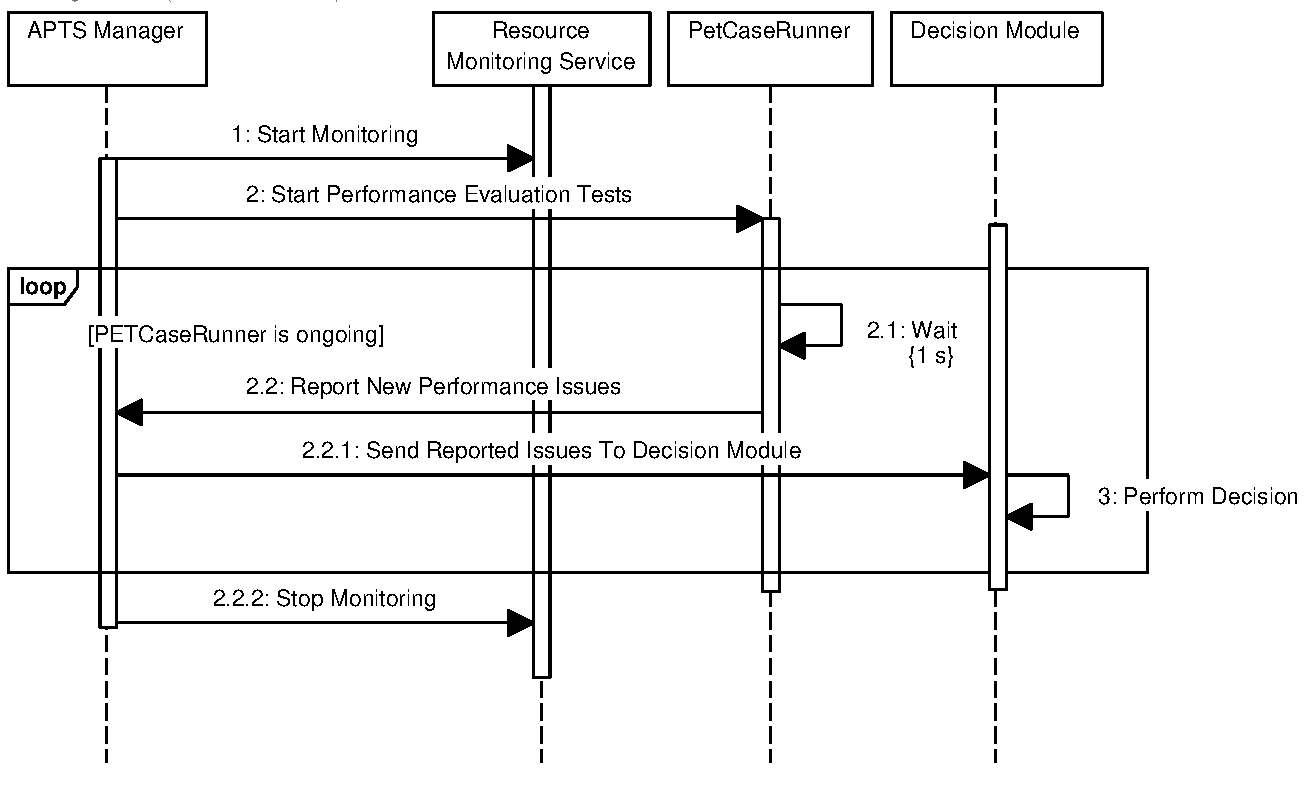
\includegraphics[width=1\textwidth]{ManagerSequenceDiagram}
\caption{\textit{Sequence Diagram presenting the APTS Manager workflow}} \label{manager}
\end{figure}


When performance tuning is started the manager starts the \textit{Resource Monitoring Service}. Next, performance evaluation test cases are executed by the \textit{PetCaseRunner}. The manager monitors any reported Performance Issues in real time and delegates every new reported issue to the \textit{Decision Module} where decision about performance tuning is made. When all PET cases performed by the \textit{PetCaseRunner} are finished the manager stops the \textit{Resource Monitoring Service} and terminates. 

\section{Solution evaluation} 

In this section the Automated Performance Tuning System will be evaluated. The evaluation of the system should confirm practical advantages of the proposed solution and reveal effectiveness under given circumstances. 

\subsection{Cache Management Evaluation}

Below experiments are focused on Cache and No Cache redundant components. The APTS should manage mentioned components in a way which provide the optimal performance of the tested application.

\subsubsection{Traffic simulation scenario} \label{trafficcachesim}

The most important concern during evaluation of the solution is traffic simulation. All decisions made by the Decision Module are based on analysis and monitoring of the incoming traffic to the application. For the case of redundant components related to cache management the traffic scenario presented in the Figure \ref{trafficcache} was implemented.

\begin{figure}[!htb]
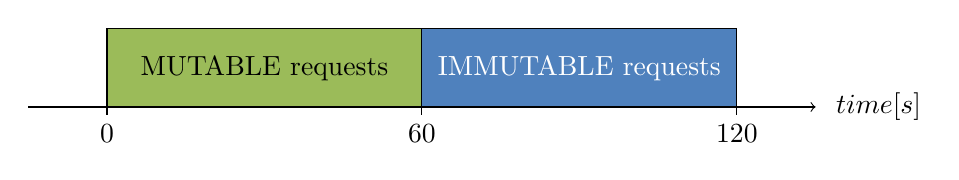
\begin{tikzpicture}
\draw[->] (0,0) -- (10,0);
\foreach \x in {1,5,9}
\draw(\x cm,3pt) -- (\x cm, -3pt);

\draw (1,0) node[below=3pt] {$0$};
\draw (5,0) node[below=3pt] {$60$};
\draw (9,0) node[below=3pt] {$120$};

\draw[fill=bblue] (5,0) rectangle (9,1);
\draw (7,0) node[above=6pt, align=center, white] {IMMUTABLE requests};

\draw[fill=ggreen] (1,0) rectangle (5,1);
\draw (3,0) node[above=6pt, align=center] {MUTABLE requests};

\draw (10.8,0) node {$time [s]$};
\end{tikzpicture}
\caption{\textit{Traffic simulation scenario for the cache management evaluation}} \label{trafficcache}
\end{figure}

The simulation takes 120 seconds and is divided in two phases. In the first 60 seconds mutable (UPDATE) requests are generated. In the second phase immutable (GET) requests are generated. The injection step of the requests is constant and is equal to 1 request per second for both phases. In the total 60 immutable and 60 mutable requests are generated during the simulation.   

\subsubsection{Environment Preparation} 

In order to prevent distortion of the results be the others managed elements (batch and threads number) only MonitorTrafficProfilePET case will be enabled during evaluation. The MonitorTrafficProfilePET was configured with parameters presented in the Table \ref{evaluationtestconf}.

\begin{table}[!htb]
\def\arraystretch{1.5}
\caption{\textit{The MonitorTrafficProfilePET case parameters}} \label{evaluationtestconf}
\begin{tabularx}{\textwidth}{X|X}

\textbf{durationInSec} & 180 \\ \hline
\textbf{monitorIntervalInSec} & 10 \\ \hline
\textbf{delayInSec:} & 10\\
\end{tabularx}
\end{table}

The initial configuration provided by the \textit{Configuration Service} during the experiment is presented in the Table \ref{cacheinitconf}.
\begin{table}[!htb]
\caption{\textit{Initial configuration}} \label{cacheinitconf}
\begin{tabularx}{\textwidth}{X|X}
\textbf{Configuration Parameter} & \textbf{Value} \\ \hline
CACHE & NO\_CACHE \\ \hline
BATCH & DIRECT\\ \hline
THREADS & T50\\
\end{tabularx}
\end{table}


\subsubsection{Control Sample} 

The goal of the control sample for this experiment is to provide reference to which results generated by the APTS can be compared. The control sample performs the same experiment as the evaluation sample but no performance tuning is made by the \textit{Decision Module}. In other words - the performance of tested application is evaluated without the APTS tuning. 
The Figure \ref{cacheCtrlGraph} presents graph generated by the Grafana platform during execution of the control sample. 

\begin{figure}[!htb]
\centering
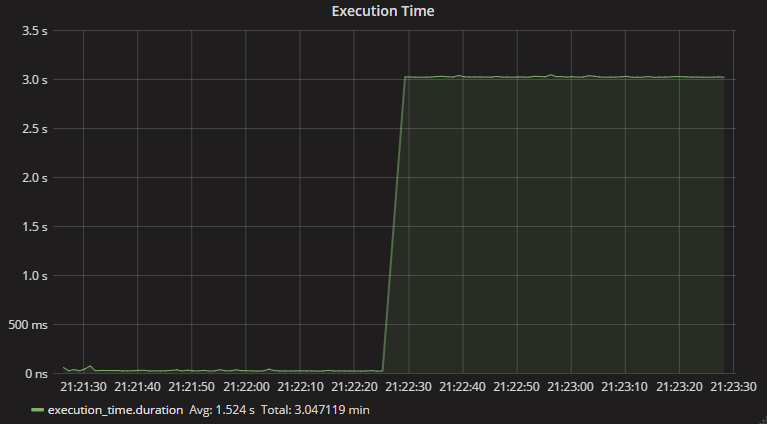
\includegraphics[width=1\textwidth]{cacheCtrl}
\caption{\textit{Screenshot from Grafana presenting graph of execution time in time}} \label{cacheCtrlGraph}
\end{figure}

According to the traffic scenario described in the Chapter \ref{trafficcachesim} two phases during experiment can be easily noticed - first one (from 21:21:25 to 21:22:25) when mutable traffic was generated and second one (from 21:22:25 to 21:23:25) when immutable traffic was generated. The execution time values are presented in the Table \ref{cacheCtrlResutls}. 

\begin{table}[!htb]
\caption{\textit{Execution time during control sample of cache evaluation}} \label{cacheCtrlResutls}
\begin{tabularx}{\textwidth}{X|X|X}
\textbf{Phase} & \textbf{Average Execution Time} & \textbf{Total Execution Time} \\ \hline
Phase 1 & 0.03s & 1.5s \\ \hline
Phase 2 & 3.02s & 183s \\ \hline
Total & 1.52s & 185s \\ 
\end{tabularx}
\end{table}

\subsubsection{Evaluation Sample} 

The goal of this evaluation sample is to evaluate the APTS solution for the cache management. The Figure \ref{cacheEvalGraph} presents graph generated by the Grafana platform during the evaluation sample. 

\begin{figure}[!htb]
\centering
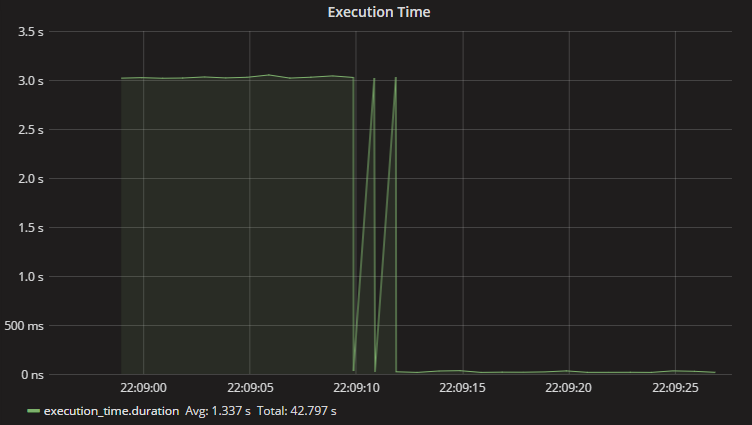
\includegraphics[width=1\textwidth]{cacheEval}
\caption{\textit{Screenshot from Grafana presenting graph of execution time in time}} \label{cacheEvalGraph}
\end{figure}

Comparing the graph from the Figure \ref{cacheEvalGraph} to control sample from the Figure \ref{cacheCtrlGraph} one can see that first phase proceeded in the same way. The execution time during the second phase was reduced after few seconds due to enabling cache by the APTS what is confirmed in the system logs: 

The APTS Manager:

\noindent\fbox{\parbox{\textwidth}{\setstretch{1.0} \texttt{\footnotesize 
2017-05-11 22:09:05.409 [main] (...) Chosen rule: EnableCacheRule\\
action: enable cache
}}}\vspace{1mm}

The Configuration Service:

\vspace{1mm}\noindent\fbox{\parbox{\textwidth}{\texttt{\footnotesize
2017-05-11 22:09:05.445 (...) Configuration of CACHE changed to value: CACHED
}}}\vspace{1mm}

The tested application:

\vspace{1mm}\noindent\fbox{\parbox{\textwidth}{\texttt{\footnotesize
2017-05-11 22:09:05.856 (...) Used redundant component: CACHED
}}}\vspace{1mm}

The execution time values are presented in the Table \ref{cacheEvalResutls}. 

\begin{table}[!htb]
\caption{\textit{Execution time during evaluation sample of cache evaluation}} \label{cacheEvalResutls}
\begin{tabularx}{\textwidth}{X|X|X}
\textbf{Phase} & \textbf{Average Execution Time} & \textbf{Total Execution Time} \\ \hline
Phase 1 & 0.035s & 2.11s \\ \hline
Phase 2 & 0.72s & 43.45ss \\ \hline
Total & 0.379s & 45.53s \\ 
\end{tabularx}
\end{table}

\subsubsection{Results Comparison} 

The Table \ref{cacheCompResutls} presents comparison of execution time between control and evaluation sample. Improvement between samples was computed using the formula: 

$Improvement = \frac{ControlSampleTimeValue}{EvaluationSampleTimeValue} \cdot 100\%$

\begin{table}[!htb]
\caption{\textit{Comparison of control and evaluation sample}} \label{cacheCompResutls}
\begin{tabularx}{\textwidth}{p{4cm}|X|X|X}
\textbf{Phase} & \textbf{Control \newline Sample} & \textbf{Evaluation Sample} & \textbf{Improvement} \\ \hline
Average Execution Time &  1.52s & 0.379s & 401\%\\ \hline
Total Execution Time &  185s & 45.53s & 406\%\\ \hline
\end{tabularx}
\end{table}

Usage of the ATPS in cache management of the tested application introduced around 400\% better performance in comparison to control sample. 

\subsection{Batch Redundant Component Evaluation}
\subsubsection{Traffic Simulation Scenario} 
\subsubsection{Environment Preparation} 
\subsubsection{Control Sample} 
\subsubsection{Evaluation Sample} 
\subsubsection{Results Comparison} 

\subsection{Threads Number Evaluation}
\subsubsection{Traffic Simulation Scenario} 
\subsubsection{Environment Preparation} 
\subsubsection{Control Sample} 
\subsubsection{Evaluation Sample} 
\subsubsection{Results Comparison} 

\subsection{Conclusions} 

\pagebreak
\clearpage
\section{References}
\renewcommand\refname{}
\begin{thebibliography}{9}

\bibitem{artperformance}
Molyneaux I., 
\textit{The Art of Application Performance Testing}, 
Sebastopol USA, O’Reilly Media, 2015.

\bibitem{javaperformance}
Oaks S., 
\textit{Java Performance: The Definitive Guide}, 
Sebastopol USA, O’Reilly Media, 2014.

\bibitem{optimizationtheory}
Rao S. S., 
\textit{Engineering Optimization Theory and Practice}, 
New Jersey USA, John Wiley \& Sons, Inc., 2009.

\bibitem{lssrarticle}
Smaalders B., 
\textit{Performance Anti-Patterns},
Queue, New York USA, vol. 4, no. 1, 2006

\bibitem{architectingperformance}
Kumar Shivakumar S. K. , 
\textit{Architecting High Performing, Scalable and Available Enterprise Web Applications},
Waltham USA, Elsevier, 2015, 101-141.

\bibitem{idealvalues}
Patel C. , Gulati R., 
\textit{Identifying Ideal Values of Parameters for Software Performance Testing},
IEEE, 2015 International Conference on Computing, Communication and Security (ICCCS), 4-5 Dec. 2015

\bibitem{comparison}
Kaur M., Kumari R.,
\textit{Comparative Study of Automated Testing Tools: TestComplete and QuickTest Pro},
International Journal of Computer Applications (0975 – 8887) Volume 24 - No.1, June 2011

\bibitem{analysisofpet}
Sharmila S., Ramadevi E.,
\textit{Analysis of Performance Testing on Web Applications},
International Journal of Advanced Research in Computer and Communication Engineering Vol. 3, Issue 3, March 2014

\bibitem{petmethodsandtools}
Sarojadevi H.,
\textit{Performance Testing: Methodologies and Tools}
Journal of Information Engineering and Applications, Vol 1, No.5, 2011.

\bibitem{howlong}
Fui-hoon F.,
\textit{A study on tolerable waiting time: how long are Web users willing to wait?}, Behaviour \& Information Technology, 23:3, 153-163, February 2007.

\bibitem{howlong}
Dang Q., Ignat C., 
\textit{Performance Evaluation of Web Based Automation Testing Tools}, Behaviour \& Information Technology, 23:3, 153-163, February 2007.

\bibitem{automaiontools}
Angmo R., Sharma M., 
\textit{Performance evaluation of web based automation testing tools}, 
5th International Conference - Confluence The Next Generation Information Technology Summit (Confluence), Noida, 2014, pp. 731-735.

\bibitem{autobugs}
Tsakiltsidis S., Miranskyy A., Mazzawi E., 
\textit{On Automatic Detection of Performance Bugs},
IEEE International Symposium on Software Reliability Engineering Workshops (ISSREW), Ottawa, ON, Canada, 2016, pp. 132-139.

\bibitem{arttest}
Myers G. J. , Sandler C.,  Badgett T.,
\textit{The art of software testing, Third Edition},
Hoboken, New Jersey, USA, John Wiley \& Sons, Inc., 2012

\bibitem{testfoundations}
Spillner A., Linz T., Schaefer H.,
\textit{Software testing foundations, Fourth Edition},
Sebastopol, California, USA, O‘Reilly Media, 2014

\bibitem{set}
Buxton J.N.,Randell  B., 
\textit{Software Engineering Techniques}, 
Rome, Italy, Report on a conference sponsored by the NATO Science Committee, p. 16., 1970

\bibitem{glassfishdoc}
\textit{GlassFish Server Open Source Edition, Performance Tuning Guide}, 
https://glassfish.java.net/docs/4.0/performance-tuning-guide.pdf,
Oracle, May 2013

\bibitem{deployerproblem}
Raghavachari M., Reimer D., Johnson R. D., 
\textit{The deployer's problem: configuring application servers for performance and reliability}, 
25th International Conference on Software Engineering, 2003. Proceedings.,2003, pp. 484-489.

\bibitem{invariantsworkloads}
Menascé D. A., Almeida V. A. F., Riedi R., Pelegrinelli F., Fonseca R., Meira W.,  
\textit{In Search of Invariants for E-Business Workloads} 
In Proceeding of Second ACM Conference on Electronic Commerce, Minneapolis, October 17-20, 2000. 

\bibitem{autotuning}
Zhang Y., Qu W., Liu A., 
\textit{Automatic Performance Tuning for J2EE Application Server Systems.}  Web Information Systems Engineering. WISE 2005. Lecture Notes in Computer Science, vol 3806. Springer, Berlin, Heidelberg

\bibitem{autoarch}
Kephart J. O., Chess D. M., 
\textit{The vision of autonomic computing}, in Computer, vol. 36, no. 1, pp. 41-50, Jan 2003.

\bibitem{autoframework}
Diaconescu A., Mos A., Murphy J., \textit{Automatic performance management in component based software systems}, International Conference on Autonomic Computing, 2004. Proceedings., 2004, pp. 214-221.

\bibitem{redundancycomponent}
Diaconescu A., \textit{A framework for using component redundancy for self-adapting and self-optimising component-based enterprise systems}, 2003, In Companion of the 18th annual ACM SIGPLAN conference on Object-oriented programming, systems, languages, and applications (OOPSLA '03). ACM, New York, NY, USA, 390-391. 

\bibitem{springperformance}
Chakraborty, A., Ditt, J., Vukotic, A., Machacek, J., \textit{Pro Spring 2.5}, Berkeley, CA, Apress, 2008, 829-855.  

\bibitem{gatling}
Gatling Load and Performance testing - Open-source load and performance testing - \textit{http://gatling.io}, (access: 15.04.2017).

\bibitem{influxdb}
InfluxData (InfluxDB) - Open Source Time Series Database for Monitoring Metrics and Events - \textit{https://www.influxdata.com}, (access: 18.04.2017).


\bibitem{junit}
JUnit - \textit{http://junit.org}, (access: 20.04.2017).

\bibitem{springaop}
Aspect Oriented Programming with Spring - \\
\textit{https://docs.spring.io/spring/docs/current/spring-framework-reference/html/aop.html}, (access: 06.05.2017).

\bibitem{nop}
Woolf B., Martin R. C., Riehle D., Buschmann F., \textit{"Null Object"}, In Pattern Languages of Program Design 3. Addison-Wesley Longman Publishing Co., Boston, USA, 1997, 5–18. 

\bibitem{grafana}
Grafana - The open platform for beautiful analytics and monitoring \textit{https://grafana.com/}, (access: 10.05.2017).

\end{thebibliography}


\end{document}
